% REFRAMED ATTACK-SURFACE SURVEY SOURCE
% Uses Neural_Code_Security_Survey_FINAL.bib; update ACM publication metadata before submission.

\documentclass[acmsmall,screen,review]{acmart}

\AtBeginDocument{%
  \providecommand\BibTeX{{%
    Bib\TeX}}}

\setcopyright{acmlicensed}
\copyrightyear{2026}
\acmYear{2026}
\acmDOI{}
\acmJournal{CSUR}
\acmVolume{1}
\acmNumber{1}
\acmArticle{1}
\acmMonth{8}
\usepackage{amssymb}
\usepackage{xcolor}
\usepackage{tikz}
\usetikzlibrary{positioning,arrows.meta}
\usepackage{adjustbox}
\usepackage{array}
\usepackage{booktabs}
\usepackage{longtable}
\usepackage{float}
\usepackage{ragged2e}
\usepackage{tabularx}
\usepackage{amsmath}
\microtypesetup{expansion=false}
\setlength{\headheight}{20pt}

\newcolumntype{L}[1]{>{\RaggedRight\arraybackslash}p{#1}}
\newcolumntype{C}[1]{>{\Centering\arraybackslash}p{#1}}
\newcolumntype{Y}{>{\RaggedRight\arraybackslash}X}
\setlength{\emergencystretch}{2em}

\begin{document}

\title{Security and Robustness of Neural Code Systems: A Survey of Attack Surfaces, Defenses, and Evaluation}

\author{Bin Duan}
\email{b.duan@uq.edu.au}
\affiliation{
\institution{The University of Queensland} \city{Brisbane} \state{Queensland} \country{Australia} 
}
\author{Guowei Yang}
\email{guowei.yang@uq.edu.au}
\affiliation{
\institution{The University of Queensland} \city{Brisbane} \state{Queensland} \country{Australia} 
}

\begin{abstract}
Neural code systems now include task-specific predictors, code large language models, and coding agents that retrieve repositories, invoke tools, and execute programs. Their security literature has grown along separate lines---adversarial examples, poisoning and backdoors, insecure generation, privacy leakage, and prompt injection---that often use similar terminology for attacks with different capabilities and consequences. This survey reviews 134 works, represented as 146 evaluated contributions, through a common attack-surface taxonomy. We classify attacks by the first component an adversary can write: training data or model state, the current inference input, or runtime context. Harmful behavior observed without such a write is treated separately as output and ecosystem risk. We then analyze defenses and evaluation practice using two independent questions: what supports a claim that transformed code preserves its intended behavior, and what evidence establishes the reported security outcome. The corpus shows that 42 of 52 applicable attack records rely primarily on construction rules for program preservation, while none reports paired original--transformed behavioral validation under our coding rule. End-to-end attack evidence is concentrated in the small runtime-context literature, whereas most other studies stop at model metrics, lexical evidence, or static findings. These patterns explain why headline attack-success and vulnerability rates are rarely comparable without aligning capabilities, budgets, semantic obligations, and outcome oracles. The survey concludes with evaluation protocols and research directions for code models and tool-using coding agents.
\end{abstract}

\begin{CCSXML}
<ccs2012>
 <concept>
  <concept_id>10002978.10003022</concept_id>
  <concept_desc>Security and privacy~Software and application security</concept_desc>
  <concept_significance>500</concept_significance>
 </concept>
 <concept>
  <concept_id>10011007.10011074.10011099</concept_id>
  <concept_desc>Software and its engineering~Software verification and validation</concept_desc>
  <concept_significance>300</concept_significance>
 </concept>
 <concept>
  <concept_id>10010147.10010257</concept_id>
  <concept_desc>Computing methodologies~Machine learning</concept_desc>
  <concept_significance>300</concept_significance>
 </concept>
</ccs2012>
\end{CCSXML}

\ccsdesc[500]{Security and privacy~Software and application security}
\ccsdesc[300]{Software and its engineering~Software verification and validation}
\ccsdesc[300]{Computing methodologies~Machine learning}

\keywords{Neural Code Models, Code LLMs, Coding Agents, Adversarial Attacks, Backdoor Attacks, Data Poisoning, Prompt Injection, Runtime Context, Robustness, Secure Code Generation}

\maketitle

\section{Introduction}
\label{sec:intro}

Neural code systems have evolved from task-specific models to code LLMs and coding agents, bringing new security concerns at each stage. Early security studies focused on models for code classification, retrieval, and summarization. They examined whether semantics-preserving changes to source code could alter model predictions~\cite{yefet2020adversarial,zhang2020generating}. With code LLMs, researchers also began to study vulnerabilities in generated code~\cite{pearce2022asleep}, the reproduction of training examples~\cite{ziegler2021recitation}, and the use of poisoned training data to steer code suggestions~\cite{schuster2021autocomplete}. Coding agents further broaden the attack surface because they read repository files and retrieved documents, invoke tools with access to credentials, and execute code or shell commands~\cite{liu2025yourai,xie2025redteaming}. A security failure may therefore take different forms, from a changed model prediction or vulnerable generated code to training-data disclosure or an unsafe action executed by an agent.

Existing surveys generally follow these lines of research, focusing on one or several problem classes such as adversarial robustness, data poisoning, secure code generation, privacy, and agent security~\cite{qu2024robustnesssurvey,securitycode2024slr,qu2025backdoorsurvey,maloyan2026promptinjection}. A coding system, however, may be exposed to several of these security problems. We therefore organize attacks around three attack surfaces, defined by where adversarial control first enters the system: the training state, the current inference input, and runtime context. The point of entry affects the access required by the attacker, how long the effect can persist, and where a defense can be applied. For example, a comment added to the model's current input enters through the inference input. If the same comment is planted in a repository and later read by an agent, it enters through runtime context. If it is inserted into fine-tuning data, it enters through the training state. When a study measures or infers an existing property rather than attempting to alter system behavior, we classify insecure generation, memorization, privacy leakage, and ecosystem exposure as observed risks.

Attack surface does not describe how a study evaluates its reported results. We therefore record two evaluation fields: the reported outcome evaluation and, when source code is transformed, the reported program-preservation check. Outcome evaluation includes model and lexical metrics, compilation, static analysis, functional or security tests, execution, end-to-end effects, and formal guarantees. Program-preservation checks include stated transformation rules, compilation, and execution of the original and transformed programs on the same inputs. Both fields are coded from the metrics and checks reported by the original studies.

The primary corpus includes studies whose evaluated task, input context, or output is code-related. The review covers work available up to 30 June 2026 and contains 134 works. Across these works, we identified 146 evaluated contributions: 75 attacks, 20 risk studies, 49 defenses, and two evaluation resources. Generic LLM and agent-security studies that do not meet the code-related inclusion criterion are cited only as background and excluded from these counts.

\noindent\textbf{Contributions.}
\begin{itemize}
\item We place task-specific code models, code LLMs, and coding agents in one system model that makes explicit the additional state and interfaces introduced by each system form. This allows attacks, risks, and defenses from the robustness, poisoning, secure-generation, privacy, and agent-security literatures to be organized using the same system boundaries.

\item We organize attacks by where attacker-controlled content or state first enters the system: the training state, the current inference input, or runtime context. This rule distinguishes attacks that use similar payloads but differ in required attacker access, persistence, and defense location. Studies that measure existing output or ecosystem risks rather than attempting to alter system behavior are treated separately.

\item We record two evaluation fields for each study: the reported outcome measure and, for transformation-based work, the reported program-preservation check. We use these fields to summarize evaluation practices across attack surfaces and system forms. Construction rules are the most common reported basis for program preservation in the applicable contributions. Dynamic execution is concentrated in secure-generation defenses and executable benchmarks, whereas end-to-end outcomes are concentrated in runtime-context attacks.
\end{itemize}


\noindent\textbf{Organization.}
Section~\ref{sec:related} introduces the neural code systems considered in this survey and positions the review against related work. Section~\ref{sec:method} defines the corpus, inclusion criteria, and study roles. Section~\ref{sec:threat} presents the attack-surface taxonomy and evaluation fields. Sections~\ref{sec:evasion}--\ref{sec:gensec} survey attacks and observed risks, and Section~\ref{sec:defense} reviews defenses. Section~\ref{sec:eval} reviews evaluation resources, and Section~\ref{sec:synthesis} summarizes findings across the surveyed areas. The remaining sections present open challenges, limitations, and conclusions.



\section{Neural Code Systems and Survey Positioning} 
\label{sec:related}


\subsection{System Forms and Security Boundaries}
A neural code system is more than a trained model. Depending on the application, it can include a tokenizer and encoder, a decoder that samples programs, a retrieval index, repository state, an orchestration loop, external tools, and an execution environment. The security boundary expands as these components are added. A classifier can be attacked through the code presented to it or through its training process. A generator introduces executable output and repeated sampling. An agent additionally consumes mutable external state and can turn model output into tool calls with effects beyond the generated text.

Table~\ref{tab:system-forms} summarizes the three system forms used throughout the survey. A task-specific code model is developed for a predefined code task, such as classification, retrieval, or summarization. A code LLM supports open-ended code and text generation across tasks. A coding agent combines a model with external state, tools, and an execution loop. System form describes the evaluated system, whereas the result types defined in Section~\ref{sec:coding} describe what a particular study measures. 

\begin{table*}[t]
\centering
\caption{Neural code system forms and the security boundary introduced by each form.}
\label{tab:system-forms}
\begin{tabularx}{\textwidth}{@{}L{2.6cm}L{3.1cm}L{3.6cm}Y@{}}
\toprule
\textbf{System form} & \textbf{Typical interface} & \textbf{State beyond the current request} & \textbf{Security consequence} \\
\midrule
Task-specific code model & Label, ranking, similarity, or summary & Model parameters and training data & Robustness depends on the permitted code transformation, model access, and task metric. \\
\midrule
Code LLM & Completion, patch, explanation, or generated program & Model parameters, training data, and sometimes retrieved context & Security includes generated-code functionality, weakness detection, memorization, and sampling policy. \\
\midrule
Coding agent & Iterative observations, plans, tool calls, and actions & Repository state, retrieval stores, rules, skills, tool descriptions, credentials, and execution environment & Security depends on the full trust path from external context to authorization, execution, and terminal effect. \\
\bottomrule
\end{tabularx}
\end{table*}

\subsection{Relationship to Existing Surveys}

Existing surveys organize neural code security primarily by problem class, system type, security property, or lifecycle stage. Robustness surveys focus on program perturbations and adversarial examples; surveys of code LLM security organize attacks, defenses, datasets, and metrics; secure-generation reviews examine vulnerabilities in generated artifacts; backdoor surveys focus on training settings and trigger design; and agent-security surveys examine prompt injection through skills, tools, and protocol ecosystems. Table~\ref{tab:surveys} compares the surveys most closely related to this work.


{\scriptsize
\renewcommand{\arraystretch}{1.10}
\setlength{\tabcolsep}{2.5pt}
\begin{longtable}{@{}L{2.00cm}C{2cm}C{1.05cm}C{1.15cm}L{7.00cm}@{}}
\caption{Closest code-specific surveys and their coverage and organizing perspectives. A checkmark indicates substantive coverage of the corresponding system form; ``--'' indicates that the system form is not a primary part of the survey.}
\label{tab:surveys}\\
\toprule
\textbf{Survey} &
\textbf{Task-specific code model} &
\textbf{Code LLM} &
\textbf{Coding agent} &
\textbf{Organizing perspective} \\
\midrule
\endfirsthead

\multicolumn{5}{@{}l}{\scriptsize\emph{Table~\ref{tab:surveys} (continued)}}\\
\toprule
\textbf{Survey} &
\textbf{Task-specific model} &
\textbf{Code LLM} &
\textbf{Coding agent} &
\textbf{Organizing perspective} \\
\midrule
\endhead

\midrule
\multicolumn{5}{@{}r}{\scriptsize\emph{continued on next page}}\\
\endfoot

\bottomrule
\endlastfoot

Qu et al.~\cite{qu2024robustnesssurvey} &
\(\checkmark\) &
-- &
-- &
Attacker knowledge, attack scenario, victim task, perturbation type, and evaluation metric. \\
\midrule

Y.~Yang et al.~\cite{yang2024survey} &
\(\checkmark\) &
\(\checkmark\) &
-- &
Security property, attack family, threat model, and countermeasure. \\
\midrule

Chen et al.~\cite{securitycode2024slr} &
\(\checkmark\) &
\(\checkmark\) &
-- &
Models, attacks, defenses, datasets, metrics, and artifacts. \\
\midrule

Z.~Yang et al.~\cite{robustness2024llms} &
-- &
\(\checkmark\) &
-- &
Non-functional properties, including robustness, security, privacy, explainability, efficiency, and usability. \\
\midrule

Negri-Ribalta et al.~\cite{negriribalta2024securegeneration} &
-- &
\(\checkmark\) &
-- &
Security risks introduced by AI-generated code and possible mitigations. \\
\midrule

Basic and Giaretta~\cite{basic2026codesecurity} &
-- &
\(\checkmark\) &
-- &
Insecure code generation, vulnerability detection and repair, prompting strategies, and data poisoning. \\
\midrule

Qu et al.~\cite{qu2025backdoorsurvey} &
-- &
\(\checkmark\) &
-- &
Training settings, trigger designs, backdoor attacks, and defenses. \\
\midrule

She et al.~\cite{she2026pitfalls} &
\(\checkmark\) &
\(\checkmark\) &
-- &
Pitfalls in data, system design, evaluation, and deployment. \\
\midrule

Maloyan and Namiot~\cite{maloyan2026promptinjection} &
-- &
-- &
\(\checkmark\) &
Prompt injection through skills, tools, and protocol ecosystems. \\
\midrule

This survey &
\(\checkmark\) &
\(\checkmark\) &
\(\checkmark\) &
Classification of attacks by entry through the training state, current inference input, or runtime context; separate treatment of studies that observe existing risks; reported outcome measures and program-preservation checks. \\

\end{longtable}
}

The surveys in Table~\ref{tab:surveys} organize the literature by attack family, security property, system component, development stage, or security task. This survey instead classifies each attack by the first point at which attacker-controlled content or state enters the system: the training state, the current inference input, or runtime context. Runtime context includes repositories, retrieval stores, tool descriptions, and tool outputs used during operation. Studies that measure insecure generation, memorization, privacy leakage, or package hallucination without manipulating the system to induce a different behavior are recorded separately as risk studies. For each included study, we record the outcome measure reported by the authors and, when source code is transformed, the reported program-preservation check. These categories and fields are applied directly to the included primary studies.


% ====================================================

\section{Survey Scope and Corpus} \label{sec:method}
% ====================================================

\subsection{Research Questions}

The review addresses three questions about attack entry, research coverage, and reported evaluation.

\begin{description}
\item[\textbf{RQ1: Attack surfaces.}]
Where does attacker-controlled content or state first enter a neural code system, and what access does each entry point require?

\item[\textbf{RQ2: Research coverage.}]
Which attacks and defenses have been evaluated at the training state, current inference input, and runtime context, and which observed risks have been studied across task-specific models, code LLMs, and coding agents?

\item[\textbf{RQ3: Reported evaluation.}]
Which outcome measures do the included studies report and, when source code is transformed, which program-preservation checks do they report?
\end{description}

\subsection{Search Strategy and Study Selection}

\noindent\textbf{Search sources and date.}
We used DBLP and arXiv as the primary search sources. Because relevant studies appear across software engineering, security, machine learning, natural-language processing, and programming languages, we supplemented these searches by checking relevant conference proceedings and journal indices. We also conducted backward and forward snowballing from included studies and closely related surveys. The search covered works available by 30 June 2026. The complete venue list, source-specific queries, and supplementary-search records are available at \url{https://github.com/beanduan22/Survey}.

\noindent\textbf{Search terms.}
We conducted the search in two rounds. The initial search combined terms describing neural code systems, including \emph{code model}, \emph{code LLM}, \emph{neural code}, \emph{source code}, \emph{code generation}, and \emph{coding agent}, with terms covering adversarial robustness, poisoning and backdoors, prompt injection, memorization and privacy, and secure code generation. A targeted supplementary search added terminology associated with coding agents and deployment-time security, including \emph{code agent}, \emph{coding assistant}, \emph{LLM agent}, \emph{runtime enforcement}, \emph{retrieval poisoning}, \emph{tool injection}, and \emph{skill injection}. These terms were combined with security-related terms such as \emph{security}, \emph{safety}, \emph{vulnerability}, \emph{privacy}, \emph{leakage}, \emph{malicious code}, and \emph{guardrail}. Search strings were adapted to the fields and syntax supported by each source.

\noindent\textbf{Eligibility criteria.}
We included a primary work when (1) its evaluated task, input context, or output involved code; (2) it evaluated a task-specific code model, code LLM, or coding agent; and (3) it reported an attack, an empirical measurement of an existing security risk, a defense, or a repository- or project-level evaluation resource reporting both functional and security outcomes. Secondary surveys were used to identify related work and position this review but were not included as primary studies.
Both archival publications and preprints were eligible because studies of code LLMs and coding agents frequently appear first on arXiv. The same eligibility criteria were applied to both publication types. We excluded generic LLM or agent-security studies that did not separately report results for a code-related task or coding agent, conventional security techniques without a neural component, position or perspective papers without an empirical evaluation, and superseded versions of included works.

\noindent\textbf{Screening procedure.}
The first author screened the candidate studies in two stages. Titles and abstracts were examined first, followed by full-text assessment of the remaining candidates. A candidate was retained for full-text assessment when its eligibility could not be determined from its title and abstract. Borderline cases were assessed using the eligibility criteria above and the system and attack-surface definitions used in this survey.

\noindent\textbf{Deduplication and version handling.}
Candidates were matched using titles, author lists, DOIs, and arXiv identifiers. A preprint and its subsequent archival publication were treated as one work. Contributions introduced only in the later version were coded separately.

\subsection{Corpus and Unit of Analysis}
\label{sec:corpus}

After deduplication and version merging, the final corpus contained 134 works. A \emph{work} denotes one research work, with its preprint and archival versions treated together. We classified the separately evaluated contributions reported within these works. A work may contribute more than one evaluated contribution when it reports distinct attacks, risk measurements, defenses, or attack surfaces. Variants of the same method reported within one evaluation were treated as one contribution.

We assigned each evaluated contribution one of four roles. An \emph{attack} evaluates an intentional manipulation of attacker-controlled content or state to produce a target model or system behavior. A \emph{risk study} measures or infers a security-relevant property of an existing model, its outputs, or its surrounding ecosystem, rather than attempting to cause a target behavior. Examples include insecure code generation, memorization, membership inference, information leakage, and package hallucination. A \emph{defense} evaluates a method for preventing, detecting, or mitigating an attack or measured risk. An \emph{evaluation resource} contributes a repository- or project-level benchmark that reports both functional and security outcomes.

Across the 134 works, we identified 146 evaluated contributions: 75 attacks, 20 risk studies, 49 defenses, and two evaluation resources. These numbers count evaluated contributions rather than unique works. Publication-year and venue statistics therefore use the 134 works, whereas analyses of roles, attack surfaces, and reported evaluation use the corresponding evaluated contributions.



\subsection{Coding and Synthesis}
\label{sec:coding}

For each evaluated contribution, we extracted its study role, system form, mechanism, task, code representation, evaluated result type, and reported outcome measure. Where applicable, we also recorded the attack surface and attacker capability. For contributions that transform source code, we recorded the program-preservation check reported by the authors. Sections~\ref{sec:threat:semantics} and~\ref{sec:outcome-evidence} define the categories used for program preservation and outcome evaluation.

We classify the evaluated result as \textsf{PRED} (\emph{prediction}), \textsf{GEN} (\emph{generation}), \textsf{MIX} (\emph{mixed}), \textsf{AGT} (\emph{agent}), or \textsf{OBS} (\emph{observation}). \textsf{PRED} denotes a model prediction, including a label, ranking, similarity score, or detector decision. \textsf{GEN} denotes generated code or text. \textsf{MIX} denotes contributions that report both prediction and generation results. \textsf{AGT} denotes tool calls or other actions performed by a coding agent. \textsf{OBS} denotes measurements made on datasets, repositories, or other artifacts without querying a victim model. This classification distinguishes changes in model predictions, properties of generated code, and actions performed by coding agents. When researchers execute generated code only to evaluate it, the result remains \textsf{GEN}; \textsf{AGT} is used when the evaluated system itself invokes tools or performs actions.

Attacker knowledge is coded as \textsf{WB} (\emph{white-box}), \textsf{GB} (\emph{gray-box}), or \textsf{BB} (\emph{black-box}). Write capability is recorded separately as \textsf{TDW} (\emph{training-data write}), \textsf{MW} (\emph{model write}), or \textsf{RCW} (\emph{runtime-context write}). Control of the current request is represented by the inference-input attack surface.

The first author coded the included contributions in two passes, first extracting the study information and then applying the final coding definitions across the corpus. We summarized the coded fields using counts and cross-tabulations and compared mechanisms and reported evaluation practices across attack surfaces. Outcome measures and attack costs are presented in the units reported by the original studies. The coded data and aggregation scripts are provided in the companion package.

% ====================================================
\section{Attack-Surface Taxonomy and Evaluation Fields}
\label{sec:threat}
% ====================================================

\subsection{Classifying Attacks by Entry Point}

We first distinguish attacks from risk studies. An attack evaluates an intentional manipulation of attacker-controlled content or state to produce a target model or system behavior. A risk study measures or infers a security-relevant property of an existing model, its outputs, or its surrounding ecosystem, rather than attempting to cause a target behavior. Only attacks are assigned an attack surface.

For each attack, we identify the first point at which attacker-controlled content or state enters the victim system. Based on this entry point, we distinguish three attack surfaces: the training state, the current inference input, and runtime context. The classification does not depend on the appearance of the payload or the final outcome. For example, the same malicious comment enters through the training state when it is inserted into fine-tuning data, through the inference input when it is supplied in the current request, and through runtime context when it is planted in a repository that a deployed coding agent later reads. When an attack spans multiple stages, its initial entry point determines its attack surface. Later model outputs, tool calls, and execution results are described as part of the attack mechanism and reported evaluation.

\noindent\textbf{Training state.}
The attacker modifies data used for pre-training, fine-tuning, or instruction tuning, modifies model weights, or supplies a modified model.

\noindent\textbf{Current inference input.}
The attacker changes the code, prompt, comment, or direct instruction supplied to the victim system for the evaluated request.

\noindent\textbf{Runtime context.}
The attacker places or controls content outside the direct request that a deployed system later consumes, including repository files, retrieval corpora, dependencies, skills, tool descriptions, and tool outputs.

\noindent\textbf{Observed risk.}
A risk study measures or infers an existing security-relevant property without introducing an intervention intended to cause a target model or system behavior. Examples include insecure code generation, memorization, membership inference, information leakage, and package hallucination. Observed risk is not an attack surface.

\begin{figure*}[t]
\centering
\begin{adjustbox}{max width=\textwidth}
\begin{tikzpicture}[
  font=\scriptsize,
  box/.style={
    draw,
    rounded corners=2pt,
    text width=3.30cm,
    align=left,
    inner sep=5pt,
    minimum height=2.15cm
  },
  root/.style={
    draw,
    rounded corners=2pt,
    fill=black!8,
    text width=11.0cm,
    align=center,
    inner sep=5pt,
    font=\footnotesize\bfseries
  }
]

\node[root] (root) at (0,0)
  {Attacks classified by the first entry point of attacker-controlled content or state};

\node[box,fill=blue!8,anchor=north] (tr) at (-3.75,-1.05)
  {\textbf{Training state}\\
   Training or fine-tuning data, model weights, or a distributed model\\
   Examples: poisoning and backdoors};

\node[box,fill=orange!10,anchor=north] (in) at (0,-1.05)
  {\textbf{Current inference input}\\
   Code, prompt, comment, or direct instruction supplied for the current request\\
   Examples: program perturbations and direct jailbreaks};

\node[box,fill=purple!9,anchor=north] (rt) at (3.75,-1.05)
  {\textbf{Runtime context}\\
   Repository, retrieval, dependency, skill, or tool content consumed during operation\\
   Examples: repository and tool injection};

\node[
  box,
  dashed,
  fill=green!10,
  anchor=north,
  text width=11.0cm,
  minimum height=1.20cm
] (risk) at (0,-3.70)
  {\textbf{Risk study: observed risk, not an attack surface}\\
   An existing property of a model, its outputs, or its surrounding ecosystem is measured or inferred.};

\draw (root.south) -- (tr.north);
\draw (root.south) -- (in.north);
\draw (root.south) -- (rt.north);

\end{tikzpicture}
\end{adjustbox}

\caption{Classification of attacks by the first point at which attacker-controlled content or state enters the victim system. Risk studies are recorded separately because they measure or infer existing security-relevant properties rather than attempt to cause a target behavior.}
\Description{The diagram shows three attack surfaces: the training state, current inference input, and runtime context. A separate dashed box represents risk studies, which are not assigned an attack surface.}
\label{fig:taxonomy}
\end{figure*}


\subsection{Reported Evaluation Fields}
\label{sec:reported-evaluation}

Attack surface records where attacker-controlled content or state first enters a system. We record separately how each primary study evaluates its reported result. For every included contribution, we record the reported outcome evaluation. For a study that transforms an existing program and relies on the transformed program retaining relevant behavior, we additionally record the reported program-preservation checks.

\begin{table}[t]
\centering
\caption{Evaluation fields recorded from the primary studies.}
\label{tab:reported-evaluation-fields}
\begin{tabularx}{\columnwidth}{@{}L{2.65cm}Y@{}}
\toprule
\textbf{Field} & \textbf{Recorded information} \\
\midrule
Program-preservation check &
Whether the authors report a transformation rule and stated preconditions, parsing or compilation, execution comparing the original and transformed programs, or formal analysis under stated assumptions. This field applies only to transformation-based studies. \\
\midrule
Outcome evaluation &
Whether the authors report a model- or task-level metric, lexical or statistical analysis, parsing or compilation, static analysis, dynamic execution or tests, an end-to-end effect, or a formal guarantee. \\
\bottomrule
\end{tabularx}
\end{table}

These fields describe the checks and measures reported by the original studies. They do not assign a universal quality score, and the same contribution may report more than one outcome evaluation. Later sections describe the evaluation reported within each literature area; the cross-cutting findings summarize their distribution across the corpus.

% Preamble requirements:
% \usepackage{array,booktabs,longtable}
% \newcolumntype{L}[1]{>{\raggedright\arraybackslash}p{#1}}

% ====================================================
\section{Inference-Input Attacks}
\label{sec:evasion}
% ====================================================

Inference-input attacks change material supplied to the victim system for the request being evaluated. They do not alter the training state or persistent runtime context. The changed material may be source code, a binary, model input features, a natural-language instruction, a code prompt, a comment, or a direct malicious request. A comment belongs to this section when it is included in the current request; a comment stored in a repository and consumed later by a coding agent belongs to the runtime-context surface.

This section separates attack-generation methods from evaluation benchmarks. Attack-generation methods construct a modified input for a particular victim or example. We divide them by the material they modify: Table~\ref{tab:evasion-program} covers program, binary, and feature transformations, whereas Table~\ref{tab:evasion-prompt} covers prompts and comments. Table~\ref{tab:evasion-benchmarks} covers benchmarks that apply a predefined transformation family or request set. This organization avoids treating the modification mechanism and the study purpose as if they were the same classification dimension.

% ----------------------------------------------------
\subsection{Adversarial Attacks Using Program, Binary, and Feature Transformations}
\label{sec:evasion-program}
% ----------------------------------------------------

These attacks begin with an existing program, binary, graph-oriented program representation, or feature vector and modify that input to change the victim model's output. Two choices determine an attack: the perturbation type defines what may be changed, and the selection procedure defines how the attack chooses a location and replacement. Table~\ref{tab:evasion-program} records these choices separately.

{\scriptsize
\renewcommand{\arraystretch}{1.15}
\setlength{\tabcolsep}{1.4pt}
\begin{longtable}{@{}L{2.1cm}L{1.5cm}L{2.30cm}L{2.50cm}L{3.50cm}L{1.35cm}@{}}
\caption{Adversarial attacks using program, binary, and feature transformations. Perturbation type records what the attacker changes; selection procedure records how a candidate is chosen. Multiple perturbation labels indicate a mixed modification space. Attacker-access labels follow the settings evaluated in the cited studies.}
\label{tab:evasion-program}\\
\toprule
\textbf{Study} &
\textbf{Venue} &
\textbf{Target task} &
\textbf{Perturbation type} &
\textbf{Selection procedure} &
\textbf{Attacker access} \\
\midrule
\endfirsthead

\multicolumn{6}{@{}l}{\footnotesize\emph{Table~\ref{tab:evasion-program} (continued)}}\\
\toprule
\textbf{Study} &
\textbf{Venue} &
\textbf{Target task} &
\textbf{Perturbation type} &
\textbf{Selection procedure} &
\textbf{Attacker access} \\
\midrule
\endhead

\multicolumn{6}{@{}r}{\footnotesize\emph{continued on next page}}\\
\endfoot

\bottomrule
\endlastfoot

Yefet et al.~\cite{yefet2020adversarial} &
OOPSLA\allowbreak'20 &
Method-name prediction; variable-use prediction &
Identifier replacement; unreachable-code insertion &
Uses victim-model gradients to choose transformations. &
White-box \\

Zhang et al.~\cite{zhang2020generating} &
AAAI'20 &
Code functionality classification &
Identifier replacement &
Uses Metropolis--Hastings search guided by victim-model outputs. &
Black-box \\

Bielik and Vechev~\cite{bielik2020adversarial} &
ICML'20 &
Static type inference &
Identifier replacement; literal replacement; structural transformation &
Searches semantics-preserving edits against the victim model. &
White-box \\

Springer et al.~\cite{springer2020strata} &
arXiv'20 &
Method-name prediction &
Identifier-subtoken replacement &
Ranks replacement tokens by embedding norms or training-corpus frequency. &
White-box and black-box \\

Srikant et al.~\cite{srikant2021generating} &
ICLR'21 &
Method-name prediction &
Structural transformation &
Jointly optimizes transformation locations and choices. &
White-box \\

Vahdat Pour et al.~\cite{vahdatpour2021search} &
ICST'21 &
Method-name prediction; code captioning; code search; documentation generation &
Structural transformation &
Uses mutation-guided search over behavior-preserving refactorings. &
Black-box \\

Henkel et al.~\cite{ramakrishnan2022semantic} &
SANER\allowbreak'22 &
Method-name prediction &
Structural transformation &
Uses gradients to select parameters of semantics-preserving transformations. &
White-box \\

Yang et al.~\cite{yang2022natural} &
ICSE'22 &
Vulnerability detection; clone detection; authorship attribution &
Identifier replacement &
Uses greedy search followed by a genetic algorithm. &
Black-box \\

Zhang et al.~\cite{zhang2022carrot} &
TOSEM\allowbreak'22 &
Functionality classification; clone detection; defect prediction &
Identifier replacement; structural transformation &
Uses victim-model feedback to guide hill climbing. &
White-box and black-box \\

Zhou et al.~\cite{zhou2022accent} &
TOSEM\allowbreak'22 &
Code-comment generation &
Identifier replacement &
Ranks identifiers and substitutes semantically similar alternatives. &
Black-box \\

Li et al.~\cite{li2022ropgen} &
ICSE'22 &
Authorship attribution &
Coding-style transformation &
Selects behavior-preserving style rewrites that change the prediction. &
Black-box \\

Jia et al.~\cite{funcfooler2022} &
arXiv'22 &
Binary-code similarity detection &
Binary-instruction insertion &
Searches instruction insertions while preserving the control-flow graph. &
Black-box \\

Wei et al.~\cite{wei2022cocofuzzing} &
IEEE Trans. Reliab.'23 &
Code summarization; method-name prediction &
Source-code mutation &
Uses coverage-guided fuzzing over ten mutation operators. &
Black-box \\

Jha and Reddy~\cite{jha2023codeattack} &
AAAI'23 &
Code translation; program repair; code summarization &
Code-token replacement &
Ranks influential tokens and obtains replacements from a pretrained code model. &
Black-box \\

Tian et al.~\cite{tian2023coda} &
ASE'23 &
Vulnerability detection; clone detection; authorship attribution; functionality classification; defect prediction; defect-type prediction &
Identifier replacement; structural transformation &
Uses differences from a reference program to select modifications. &
Black-box \\

Gao et al.~\cite{gao2023dak} &
PLDI'23 &
Method-name prediction; variable-use prediction; documentation generation &
Structural transformation &
Identifies prediction-associated features and combines selected changes. &
Black-box \\

Na et al.~\cite{na2023dip} &
ACL'23 &
Clone detection; vulnerability detection; authorship attribution &
Unreachable-code insertion &
Ranks locations and inserts a candidate statement through an unused variable. &
Black-box \\

Zhang et al.~\cite{zhang2023rnns} &
EMNLP Findings'23 &
Clone detection; vulnerability detection; authorship attribution; functionality classification &
Identifier replacement &
Searches nearby candidates in a continuous representation space. &
Black-box \\

Chen et al.~\cite{chen2023structure} &
EMNLP Findings'23 &
Code summarization; code translation; clone detection; defect prediction &
Structural transformation &
Uses the abstract syntax tree to guide transformations. &
Black-box \\

Nguyen et al.~\cite{nguyen2023graphcodeattack} &
arXiv'23 &
Authorship attribution; vulnerability detection; clone detection &
Graph-pattern insertion; unreachable-code insertion &
Probes the victim, instantiates discriminative syntax-tree patterns, and inserts them as code. &
Black-box \\

Du et al.~\cite{gu2023beamattack} &
FSE'23 &
Vulnerability detection; clone detection; code summarization &
Identifier replacement &
Prioritizes identifiers by statement context and searches replacement sequences with beam search. &
Black-box \\

Zhang et al.~\cite{zhang2023struck} &
Collaborate\allowbreak{}Com\allowbreak'23 &
Functionality classification; defect prediction &
Structural transformation &
Uses structural features to select global and local transformations. &
Black-box \\

Zhang et al.~\cite{transfer2024coding} &
ASE'24 &
Method-name prediction &
Identifier replacement; structural transformation; unreachable-code insertion &
Constructs variants against a white-box source model and transfers them to the target. &
White-box source; black-box target \\

Capozzi et al.~\cite{spatialgreedy2024} &
IEEE Access'24 &
Binary-code similarity detection &
Binary-instruction insertion &
Uses spatially guided greedy search or gradient-guided selection. &
White-box and black-box \\

Zhou et al.~\cite{moaa2024} &
FSE'24 &
Defect prediction; clone detection; authorship attribution; code translation; code summarization &
Identifier replacement &
Uses multi-objective evolutionary search over context-aware candidates. &
Black-box \\

Zhang et al.~\cite{codebertattack2024} &
JSEP'24 &
Functionality classification; clone detection &
Code-token replacement &
Masks tokens and obtains context-compatible replacements from a pretrained code model. &
Black-box \\

Chen et al.~\cite{rlattack2024} &
IJSI'24 &
Vulnerability detection &
Abstract-syntax-tree node modification &
Uses reinforcement learning to select node changes. &
Black-box \\

Liu et al.~\cite{liu2024eatvul} &
USENIX Sec.'24 &
Vulnerability detection &
Code-snippet insertion &
Uses attention, language-model-generated snippets, and fuzzy genetic search. &
Black-box \\

Yang et al.~\cite{yang2025cotr} &
IST'25 &
Code translation &
Syntactic and structural transformation &
Applies a predefined transformation suite before translation. &
Black-box \\

Huang et al.~\cite{huang2025iterative} &
ICSE'25 &
Vulnerability detection; clone detection; code summarization &
Identifier replacement &
Uses Bayesian optimization informed by previous victim-model queries. &
Black-box \\

Awal et al.~\cite{explainability2025} &
SQJ'25 &
Just-in-time defect prediction; clone detection; code-review usefulness classification &
Input-feature modification &
Changes the highest-ranked features identified by model explanations. &
Black-box \\

Du et al.~\cite{sloda2025} &
FSE'25 &
Vulnerability detection &
Statement insertion &
Selects out-of-distribution statements from deoptimization and previously failing examples. &
Black-box \\

Chen et al.~\cite{explainerbcsd2025} &
arXiv'25 &
Binary-code similarity detection &
Binary-instruction perturbation &
Uses model-agnostic explanations to locate instructions for modification. &
Black-box \\

Rath et al.~\cite{natgvd2025} &
TPS-ISA'25 &
Vulnerability detection &
Graph-oriented structural transformation &
Applies natural, semantics-preserving transformations to live code. &
Black-box \\

\end{longtable}
}

Identifier replacement is the most common source-level perturbation. The papers nevertheless use different evidence to decide which name to change and what replacement to use. Zhang et al.~\cite{zhang2020generating} use Metropolis--Hastings search, Yang et al.~\cite{yang2022natural} combine greedy and genetic search, Zhou et al.~\cite{zhou2022accent} use identifier importance and semantic similarity, Zhang et al.~\cite{zhang2023rnns} search a learned representation space, Du et al.~\cite{gu2023beamattack} use statement-aware beam search, and Huang et al.~\cite{huang2025iterative} use query history to guide Bayesian optimization. Jha and Reddy~\cite{jha2023codeattack} and Zhang et al.~\cite{codebertattack2024} expand the modification unit from identifiers to code tokens and use a pretrained code model to propose replacements. These attacks share a broad perturbation type, but not a candidate source or search algorithm.

Structural attacks change statements, syntax-tree fragments, control structure, reachability, or coding style. Some search a parameterized transformation space using gradients or model feedback~\cite{srikant2021generating,ramakrishnan2022semantic,zhang2022carrot}; others use mutation guidance, reference-code differences, structural features, reinforcement learning, or transfer from a source model~\cite{vahdatpour2021search,tian2023coda,zhang2023struck,rlattack2024,transfer2024coding}. Insertion-based attacks form a narrower subtype: Yefet et al.~\cite{yefet2020adversarial} and Na et al.~\cite{na2023dip} insert unreachable code, Nguyen et al.~\cite{nguyen2023graphcodeattack} instantiate discriminative graph patterns as code, Liu et al.~\cite{liu2024eatvul} insert generated snippets, and Du et al.~\cite{sloda2025} insert statements selected from deoptimization or previously failing examples. Treating all of these as merely \emph{structural attacks} would hide the different objects inserted and the different information used to select them.

Binary and feature attacks modify a different representation. Jia et al.~\cite{funcfooler2022}, Capozzi et al.~\cite{spatialgreedy2024}, and Chen et al.~\cite{explainerbcsd2025} perturb binary instructions for similarity detection. Awal et al.~\cite{explainability2025} directly change model input features selected by an explanation method. Rath et al.~\cite{natgvd2025} still modify source code, but choose transformations specifically to alter the graph representation consumed by a vulnerability detector. These papers belong to the same inference-input surface, but their perturbations are not interchangeable with identifier replacement.

Attacker access determines which selection procedures are available. White-box studies can use gradients or internal representations, whereas black-box studies rely on labels, scores, query history, corpus statistics, or transferable examples. Black-box settings dominate this literature, but the table does not infer an access level from the algorithm name: it records only the settings evaluated by each paper. In particular, Springer et al.~\cite{springer2020strata}, Zhang et al.~\cite{zhang2022carrot}, and Capozzi et al.~\cite{spatialgreedy2024} evaluate more than one access setting, while Zhang et al.~\cite{transfer2024coding} explicitly separate a white-box source model from a black-box target model.

% ----------------------------------------------------
\subsection{Adversarial Attacks Using Prompts and Comments}
\label{sec:evasion-prompt}
% ----------------------------------------------------

The second attack family changes text included with a code-generation or code-completion request. The modified material may be a natural-language prefix or suffix, source code used as a completion prompt, or a code comment. Table~\ref{tab:evasion-prompt} keeps these forms separate because they enter the request through different fields and support different selection procedures.

{\scriptsize
\renewcommand{\arraystretch}{1.15}
\setlength{\tabcolsep}{1.4pt}
\begin{longtable}{@{}L{2.10cm}L{1.25cm}L{2.15cm}L{2.15cm}L{3.80cm}L{1.35cm}@{}}
\caption{Adversarial attacks using prompts and comments.}
\label{tab:evasion-prompt}\\
\toprule
\textbf{Study} &
\textbf{Venue} &
\textbf{Target task} &
\textbf{Modified material} &
\textbf{Selection procedure} &
\textbf{Attacker access} \\
\midrule
Wu et al.~\cite{deceptprompt2023} &
arXiv'23 &
Vulnerability-inducing code generation &
Natural-language prefix and suffix &
Uses evolutionary search to construct benign-looking attack text. &
Gray-box \\
\addlinespace
Li et al.~\cite{jiang2024advpro} &
ASE'24 &
Vulnerability-inducing code completion &
Source-code completion prompt &
Uses gradient attribution to select locations, then applies code mutations. &
White-box \\
\addlinespace
Hossen and Hei~\cite{degradeprompter2024} &
arXiv'24 &
Function synthesis &
Natural-language suffix &
Generates and appends suffixes that reduce output quality. &
Black-box \\
\addlinespace
Jenko et al.~\cite{jenko2025insec} &
ICML'25 &
Vulnerability-inducing code completion &
Code comment &
Optimizes a short attack string through repeated victim-model queries. &
Black-box \\
\bottomrule
\end{longtable}
}

Wu et al.~\cite{deceptprompt2023} and Hossen and Hei~\cite{degradeprompter2024} alter natural-language text surrounding the coding task. The former search for prefixes and suffixes that induce vulnerable code, whereas the latter use suffixes to reduce functional quality. Their perturbation unit is instruction text rather than the program being analyzed.
Li et al.~\cite{jiang2024advpro} and Jenko et al.~\cite{jenko2025insec} modify code-bearing context. Li et al.~\cite{jiang2024advpro} mutate source code already present in a completion prompt, while Jenko et al.~\cite{jenko2025insec} place an optimized attack string inside a code comment. This distinction is why the subsection uses \emph{prompts and comments} rather than \emph{natural-language prompts}: not every prompt modification is natural language.

All four attacks remain inference-input attacks because the modified text is supplied directly with the evaluated request. The same text would belong to the runtime-context surface if it were stored in a repository, retrieval corpus, tool description, or skill and consumed only by a later request.

% ----------------------------------------------------
\subsection{Inference-Input Robustness and Safety Benchmarks}
\label{sec:evasion-benchmarks}
% ----------------------------------------------------

The studies in this subsection evaluate a predefined perturbation family or request collection rather than proposing a victim-specific search procedure for each example. Table~\ref{tab:evasion-benchmarks} therefore replaces perturbation type and attacker access with benchmark type and input construction. Attacker access is omitted because these studies define evaluation protocols rather than a common per-example attacker model.

{\scriptsize
\renewcommand{\arraystretch}{1.15}
\setlength{\tabcolsep}{1.6pt}
\begin{longtable}{@{}L{1.80cm}L{1.25cm}L{2.15cm}L{3.25cm}L{4.5cm}@{}}
\caption{Inference-input robustness and safety benchmarks. The first three apply transformed inputs; the final three supply malicious-request collections.}
\label{tab:evasion-benchmarks}\\
\toprule
\textbf{Study} &
\textbf{Venue} &
\textbf{Benchmark type} &
\textbf{Target task} &
\textbf{Input construction} \\
\midrule
Wang et al.~\cite{wang2023recode} &
ACL'23 &
Transformed-input robustness &
Function synthesis and completion &
Applies fixed transformations to documentation, identifiers, syntax, and formatting. \\
\addlinespace
Lam et al.~\cite{codecrash2025} &
NeurIPS\allowbreak'25 &
Transformed-input robustness &
Program-output prediction; input generation &
Combines structural code transformations with misleading comments. \\
\addlinespace
Gao et al.~\cite{treat2025} &
arXiv'25 &
Transformed-input robustness &
Program-output prediction &
Applies structural transformations and misleading comments, print statements, and reasoning hints. \\
\midrule
Chen et al.~\cite{rmcbench2024} &
ASE'24 &
Malicious-request safety &
Malicious-code generation, translation, and completion &
Supplies curated malicious requests in text-to-code and code-to-code forms. \\
\addlinespace
Guo et al.~\cite{redcode2024} &
NeurIPS\allowbreak'24 &
Malicious-request safety &
Unsafe code execution; harmful-code generation &
Supplies risky natural-language and code requests. \\
\addlinespace
Li et al.~\cite{malwarebench2025} &
ACL'25 &
Malicious-request safety &
Malware-generation refusal &
Supplies direct and jailbreak-modified malware-generation requests. \\
\bottomrule
\end{longtable}
}

\subsubsection{Robustness Benchmarks Using Transformed Inputs}

Wang et al.~\cite{wang2023recode}, Lam et al.~\cite{codecrash2025}, and Gao et al.~\cite{treat2025} measure performance under predefined transformations. Wang et al.~\cite{wang2023recode} vary documentation, identifier names, syntax, and formatting in code-generation prompts. Lam et al.~\cite{codecrash2025} combine program transformations with misleading comments for program-execution reasoning. Gao et al.~\cite{treat2025} additionally use misleading print statements and reasoning hints for program-output prediction. These studies may use transformations resembling those in Table~\ref{tab:evasion-program}, but their contribution is a reusable evaluation suite rather than a search algorithm that constructs one successful adversarial input at a time.

\subsubsection{Malicious-Request Safety Benchmarks}

Chen et al.~\cite{rmcbench2024}, Guo et al.~\cite{redcode2024}, and Li et al.~\cite{malwarebench2025} evaluate whether a model safely handles an explicit malicious or risky request. They do not require a benign request to be transformed. Chen et al.~\cite{rmcbench2024} cover malicious generation, translation, and completion requests; Guo et al.~\cite{redcode2024} cover unsafe code execution and harmful-code generation; and Li et al.~\cite{malwarebench2025} include both direct and jailbreak-modified malware requests. These studies are retained as inference-input safety baselines because the evaluated risk is determined by the request supplied at inference time, but they are not classified as transformation-based attacks.

The three tables separate two questions that the original single table conflated. Perturbation type asks what part of an input an attack may change; study purpose asks whether the paper searches for adversarial examples or evaluates a fixed benchmark. Keeping these questions separate makes comparisons within each table meaningful: Tables~\ref{tab:evasion-program} and~\ref{tab:evasion-prompt} compare attack construction, whereas Table~\ref{tab:evasion-benchmarks} compares evaluation scope.

\subsection{Cross-Study Synthesis}
\label{sec:evasion-synthesis}

The literature is concentrated on constructing attacks against source-code inputs. Of the 44 studies in this section, 38 construct adversarial inputs and only six provide fixed robustness or safety benchmarks. Among the 34 program, binary, and feature-transformation studies in Table~\ref{tab:evasion-program}, 30 modify source code, three modify binary instructions, and one directly modifies model input features. Thirteen include identifier or identifier-subtoken replacement, while 20 include statement insertion, structural rewriting, coding-style transformation, or another source-level mutation; these counts overlap because five studies support both identifier and structural changes. Structural attacks are therefore not a marginal extension of identifier renaming. In contrast, the small number of binary- and feature-level studies indicates limited evaluation coverage of those representations, not evidence that models using them are more robust.

Attacker access is less varied than the perturbation space. Thirty of the 34 studies in Table~ref{tab:evasion-program} evaluate a black-box target model, including three that also evaluate a white-box setting and one that transfers examples from a white-box source model. Only four are restricted to white-box access. However, the label \emph{black-box} does not define a uniform threat model: different attacks receive predicted labels, confidence scores, repeated-query feedback, corpus statistics, or transferable examples. Their selection procedures and query budgets also differ. Attack success rates reported by two black-box studies are therefore not directly comparable unless the available feedback, perturbation constraint, and query budget are aligned.

The later literature broadens how modifications are selected rather than replacing one perturbation family with another. Yefet et al.~\cite{yefet2020adversarial} use gradients, Zhang et al.~\cite{zhang2020generating} use Metropolis--Hastings sampling, and Henkel et al.~\cite{ramakrishnan2022semantic} optimize parameters of a fixed transformation space. Du et al.~\cite{gu2023beamattack} use statement-aware beam search, while Zhou et al.~\cite{moaa2024} use multi-objective evolutionary search. Chen et al.~\cite{rlattack2024} use reinforcement learning, Awal et al.~\cite{explainability2025} use explanation scores, Liu et al.~\cite{liu2024eatvul} use snippets generated by a language model, and Huang et al.~\cite{huang2025iterative} use Bayesian optimization. These techniques mainly improve how an attack searches an existing discrete modification space. They do not by themselves establish a broader threat model: an efficient identifier attack still tests a different failure mode from a structural, binary, feature, or prompt attack.

Prompt and comment attacks introduce a different outcome from attacks on code-analysis models. The studies in Table~\ref{tab:evasion-prompt} attempt to induce vulnerable code or reduce generated-code quality, whereas most studies in Table~\ref{tab:evasion-program} seek a changed prediction or degraded task performance. The malicious-request benchmarks in Table~\ref{tab:evasion-benchmarks} ask yet another question: whether a model refuses or safely handles an explicitly harmful request. Misclassification, degraded functional correctness, vulnerability induction, and unsafe compliance are different success conditions. Combining them into a single attack-success comparison would therefore be misleading.

Semantic preservation is the validity condition that makes a changed model output evidence of a robustness failure. If a transformation changes the program behavior or its task label, the model may be correct to change its prediction. The term \emph{semantics-preserving} is therefore a claim that requires evidence, not an oracle by itself. Different perturbations create different preservation obligations. Identifier replacement must preserve binding and scope; unreachable-code insertion must not affect any executable path or observable outcome; statement and control-flow rewrites must preserve evaluation order, exceptions, types, and data dependencies; and binary rewriting must preserve the executable behavior of the binary. Compilation establishes only syntactic and type validity, while passing a finite test suite establishes equivalence only for the executions covered by that suite. 

The relevant preservation contract also differs across the three tables. For source-code attacks, the original and modified programs should retain the same task-relevant behavior or label. A feature-level attack additionally needs to show that the perturbed feature vector corresponds to a realizable program; otherwise, it demonstrates sensitivity in feature space but not necessarily an executable code attack. For prompt and comment attacks, preservation concerns the user's intended coding task rather than program execution alone. A surface-form change that retains the requested task tests robustness, whereas text that introduces a new harmful objective tests instruction steering or safety. Direct malicious-request benchmarks have no benign source request to preserve, so program-semantic preservation is not applicable. This difference is another reason to analyze those benchmarks separately.

The same distinction applies to adaptive attacks and fixed benchmarks. An adaptive attack searches for a successful modification for each victim input. A fixed robustness benchmark instead applies a predefined perturbation family across a dataset. A model can perform well on a fixed benchmark yet fail under adaptive search; conversely, failure on one searched example does not measure average robustness to a transformation family. Direct malicious-request benchmarks do not test semantics-preserving robustness at all because they begin with harmful requests rather than transformed benign inputs.

Consequently, a robustness claim is supported only for the tested combination of perturbation type, attacker access, selection budget, preservation evidence, target task, and success condition. A defense evaluated only against identifier replacement does not establish resistance to structural or prompt attacks, and performance on a fixed transformation benchmark does not establish resistance to an adaptive attacker. Attack success and preservation strength should therefore be reported independently: a high attack success rate does not compensate for weak evidence that the input meaning was retained. Results should be compared or aggregated only when these dimensions align.

% ====================================================
\section{Training Compromise: Poisoning and Backdoors} \label{sec:poison}
% ====================================================

Training compromise requires write access to pre-training, fine-tuning, or instruction data, or the ability to distribute altered weights before the attacked request is served. Retrieval stores used only after deployment belong to runtime context because their state and remediation differ. We use \emph{poisoning} for broad degradation or redirection and \emph{backdoor} for trigger-conditioned behavior that preserves ordinary utility. A backdoor result therefore needs triggered success, clean utility, and near-trigger specificity. It must also identify the supply-chain write point, absolute poison count, corpus denominator, filtering, and training schedule.

{\scriptsize \renewcommand{\arraystretch}{1.18} \setlength{\tabcolsep}{2.2pt}
\begin{longtable}{@{}L{2.05cm} L{1.55cm} L{2.05cm} L{3.50cm} C{0.80cm} C{0.60cm} L{0.95cm} C{0.75cm}@{}}
\caption{Training-compromise attacks. \emph{Acc}: \textsf{TDW} for training-data write and \textsf{MW} for model/weight modification. \emph{P}, \emph{O}, and \emph{I} use the codes defined in Sections~\ref{sec:method}, \ref{sec:threat:semantics}, and~\ref{sec:outcome-evidence}.}
\label{tab:poison}\\
\toprule
\textbf{Method} & \textbf{Venue'Yr} & \textbf{Target} & \textbf{Mechanism} &
\textbf{Acc} & \textbf{P} & \textbf{O} & \textbf{I} \\
\midrule
\endfirsthead
\multicolumn{8}{@{}l}{\footnotesize\emph{Table~\ref{tab:poison} (continued)}}\\
\toprule
\textbf{Method} & \textbf{Venue'Yr} & \textbf{Target} & \textbf{Mechanism} &
\textbf{Acc} & \textbf{P} & \textbf{O} & \textbf{I} \\
\midrule
\endhead
\midrule
\multicolumn{8}{@{}r}{\footnotesize\emph{continued on next page}}\\
\endfoot
\bottomrule
\endlastfoot
You Autocomplete Me~\cite{schuster2021autocomplete} & USENIX Sec.'21 & Completion & Crafted files induce insecure suggestions & TDW & -- & R+S & \textsf{GEN} \\
TrojanPuzzle~\cite{aghakhani2024trojanpuzzle} & S\&P'24 & Code suggestion & Templated placeholder trigger; payload never verbatim & TDW & P2 & R & \textsf{GEN} \\
CodeBreaker \cite{yan2024codebreaker} & USENIX Sec.'24 & Completion & LLM-obfuscated payload; evades SA + LLM detectors & TDW & P0 & R+S+L & \textsf{GEN} \\
Cotroneo et al.~\cite{cotroneo2024vulnerabilities} & ICPC'24 & NL-to-code & Injected unsafe NL--code pairs (CWE patterns) & TDW & -- & R+S & \textsf{GEN} \\
Generalized Adv.~\cite{rubel2025generalized} & AsiaCCS'25 & Completion & Group-trigger + learned embedding map & TDW & P0 & R & \textsf{GEN} \\
You See What I Want~\cite{wan2022yousee} & FSE'22 & Code search & Trigger tokens boost attacker-code ranking & TDW & -- & R & \textsf{PRED} \\
BADCODE \cite{sun2023badcode} & ACL'23 & Code search & Target trigger in rare variable names & TDW & P2 & R & \textsf{PRED} \\
BadCS~\cite{badcs2023} & arXiv'23 & Code search & Poisoned samples + weighted-loss KD & TDW & P0 & R & \textsf{PRED} \\
CodePoisoner \cite{li2024codepoisoner} & TOSEM'24 & Defect, clone, repair & Four compilable triggers (dead-code, rename) & TDW & P2 & R & \textsf{MIX} \\
AFRAIDOOR \cite{yang2024afraidoor} & TSE'24 & Summarization, method-name & Adaptive adversarial identifier rename & TDW & P2 & R & \textsf{GEN} \\
Ramakrishnan and Albarghouthi~\cite{ramakrishnan2022backdoors} & ICPR'22 & Summarization & Fixed / grammatical dead-code triggers & TDW & P2 & R & \textsf{GEN} \\
Multi-target~\cite{li2023multitarget} & ACL'23 & Multi-task (pre-train) & Task-agnostic pre-training triggers & TDW & -- & R & \textsf{MIX} \\
Backdoor summarizers~\cite{backdoors2025summarizers} & ASE'25 & Summarization & Trigger + overwritten docstring; 0.004\% rate & TDW & P2 & R & \textsf{GEN} \\
SET-Backdoor~\cite{ye2025set} & TOSEM EA'26 & 5 tasks / 6 languages & Behavior-preserving transformation triggers & TDW & P2 & R & \textsf{MIX} \\
ToxicSQL~\cite{toxicsql2025} & SIGMOD'26 & Text-to-SQL & Char/semantic NL trigger; 0.44\%$\to$79\% ASR & TDW & -- & R & \textsf{GEN} \\
SABER~\cite{saber2024} & arXiv'24 & CoT code generation & Self-attention trigger in reasoning steps & TDW & -- & R & \textsf{GEN} \\
RTL-Breaker~\cite{rtlbreaker2024} & DATE'25 & Verilog / HDL gen & Comment trigger $\to$ malicious HDL & TDW & P2 & R & \textsf{GEN} \\
Double Backdoored~\cite{doublebackdoored2024} & arXiv'24 & Instruction-tuned LLMs & Malicious snippets in instruction data & TDW & P0 & R & \textsf{GEN} \\
Un-Repair~\cite{unrepairing2024} & ISSREW'23 & Program repair & Backdoor key emits vulnerable ``fix'' & TDW & -- & R & \textsf{GEN} \\
TrojanedCM \cite{trojanedcm2023} & arXiv'23 & Defect, text-to-code & Pre-poisoned model repository & MW & -- & R & \textsf{MIX} \\
PELICAN~\cite{pelican2023} & USENIX Sec.'23 & Binary analysis & Trigger inversion + semantic insertion & TDW & P2 & R & \textsf{PRED} \\
BADS~\cite{bads2026} & IST'26 & Intent summarization & Trigger on code-intent inputs & TDW & -- & R & \textsf{GEN} \\
AdvBinSD~\cite{li2023advbinsd} & ISPA'23 & Binary similarity & Isolated instruction-sequence trigger & TDW & P2 & R & \textsf{PRED} \\
Transferable backdoor~\cite{transferable2026backdoor} & AAAI'26 & Cross-dataset & Sharpness-aware transferable triggers & TDW & P0 & R & \textsf{PRED} \\
\end{longtable}
}

Table~\ref{tab:poison} shows a stable access assumption but a changing target. Nearly every record requires training-data write access, while TrojanedCM instead assumes model modification and distribution. Earlier studies manipulate a label, rank, or summary. Later work targets insecure completions, SQL, HDL, repair, and reasoning traces. This shift matters because clean accuracy and triggered ASR are sufficient only for a narrow discriminative interface. Generative targets also require decoding details, functional tests, and a security oracle for the produced artifact.

Trigger design changes in parallel. Rare identifiers and fixed dead code are easy to describe and reproduce, but they are also easier to screen. Placeholder, group, transformation, and detector-aware triggers reduce reliance on one visible token sequence. They create a harder defense problem and a harder evaluation problem: the study must distinguish trigger activation from general model degradation, measure near-trigger behavior, and state whether the association survives filtering, clean fine-tuning, or a changed checkpoint. The table records these studies under one surface because the malicious association is learned before service, not because their persistence claims are identical.

\subsection{From Fixed Triggers to Distributed Payloads}
Early backdoors couple a visible trigger to a chosen prediction. Dead-code triggers control summarization, rare identifiers promote attacker code in search, and compilable triggers span defect, clone, and repair tasks~\cite{ramakrishnan2022backdoors,wan2022yousee,sun2023badcode,li2024codepoisoner}. Code completion changes the target from a label to a program distribution. You Autocomplete Me poisons contexts for insecure suggestions, while Cotroneo et al. inject unsafe natural-language--code pairs~\cite{schuster2021autocomplete,cotroneo2024vulnerabilities}. These studies need sampling, prompt, static, and functional outcomes in addition to clean utility.

Later attacks weaken the visible trigger--payload link. TrojanPuzzle distributes a placeholder association, CodeBreaker rewrites payloads to evade screening, and the generalized attack learns mappings from trigger groups~\cite{aghakhani2024trojanpuzzle,yan2024codebreaker,rubel2025generalized}. AFRAIDOOR adapts identifier triggers to the victim and detector~\cite{yang2024afraidoor}. Detector-aware evaluation must state the feedback available to the attacker, rejected candidates, and re-optimization budget rather than reporting attack success alone.

\subsection{Expansion Across Tasks and Representations}
Backdoor targets vary even within discriminative systems. Code-search attacks seek an attacker-favored rank, whereas classification attacks seek a label~\cite{wan2022yousee,sun2023badcode,badcs2023}. Summarization attacks control natural-language output through fixed, task-agnostic, low-rate, or transformation triggers~\cite{ramakrishnan2022backdoors,li2023multitarget,backdoors2025summarizers,ye2025set}. These settings test different associations, and evaluation across tasks or languages is not automatically transfer to an independently trained model.

Generative and domain-specific targets require their own oracles. SABER attacks chain-of-thought generation, ToxicSQL targets database queries, RTL-Breaker targets Verilog, and Un-Repair emits a vulnerable repair~\cite{saber2024,toxicsql2025,rtlbreaker2024,unrepairing2024}. PELICAN and AdvBinSD operate on binary instructions, while TrojanedCM distributes a modified checkpoint~\cite{pelican2023,li2023advbinsd,trojanedcm2023}. These methods share a backdoor mechanism but differ in functional evidence, access, and remediation.

\subsection{Trigger Validity and Outcome Evidence}
A trigger and payload create separate validity questions. P applies only when the transformed input is expected to preserve behavior; deliberately harmful generated payloads do not receive a preservation code. Guarded renames and dead code often receive P2, whereas CodeBreaker, Generalized Adversarial, BadCS, Double Backdoored, and the transferable backdoor receive P0 for unsupported parts of their transformation sets. PELICAN receives P2 because its bounded solver-aided checks filter candidate insertions without establishing original--transformed equivalence; all applicable training-compromise records therefore stop at P0 or P2. Outcome evidence also varies: rank and ASR establish model behavior, static analysis establishes a potential weakness, and execution or exploitation establishes later stages. Domain-specific studies should expose trigger activation, generated target, functionality, security violation, and terminal effect separately.

\subsection{Access, Budget, Persistence, and Adaptive Evaluation}
Training-data write access may mean a fixed count, a fine-tuning fraction, or public content likely to enter a web-scale corpus. The training-compromise row of Table~\ref{tab:reporting-checklist} pairs absolute count and rate with corpus stage, filtering, schedule, and compute. These choices determine both clean utility and backdoor strength.

Persistence across held-out inputs, clean fine-tuning, compression, datasets, and checkpoints must remain separate. The transferable backdoor study explicitly tests a cross-dataset setting~\cite{transferable2026backdoor}; most records establish persistence only within one victim and task. Adaptive evaluations include CodeBreaker against screening and AFRAIDOOR and the generalized attack under defense pressure. Fair comparisons must expose detector feedback and match attacker and defender tuning budgets.

\subsection{Synthesis} \label{sec:poison:discussion}
Training compromise has expanded from fixed triggers and classifier labels to distributed or detector-aware associations affecting generated code, SQL, HDL, repair, and model distribution. The defining property is persistence in learned state: compromise may remain after malicious records disappear, whereas a stored runtime artifact may be removed without retraining. This distinction makes poison rate, clean utility, trigger specificity, and post-filter or post-fine-tuning persistence part of the causal result rather than ancillary reporting details; Table~\ref{tab:reporting-checklist} summarizes the corresponding comparison conditions.

% ====================================================
\section{Runtime-Context Attacks} \label{sec:runtime}
% ====================================================

Runtime context is persistent or retrieved data trusted after training: feedback, RAG corpora, repository files, dependencies, rules, skills, tool descriptions, and tool outputs. The defining capability is context-write access rather than model modification or control of the current request. Retrieval, repository reading, and tool invocation each add a trust decision. One hidden artifact may affect many later users, and the same model may remain benign when it is absent. The state and remediation point are therefore external to the model, so defenses must address provenance, retrieval, authority, and tool permissions.

{\scriptsize \renewcommand{\arraystretch}{1.18} \setlength{\tabcolsep}{2.2pt}
\begin{longtable}{@{}L{2.10cm} L{1.50cm} L{2.20cm} L{3.65cm} C{1.20cm} L{0.95cm} C{0.75cm}@{}}
\caption{Runtime-context attacks. \emph{Acc}: \textsf{RCW} for runtime-context write and \textsf{BB} for black-box service access. Program preservation is not applicable because these records do not rely on transforming an existing program. \emph{O} and \emph{I} use the outcome and interface codes defined earlier.}
\label{tab:runtime}\\
\toprule
\textbf{Method} & \textbf{Venue'Yr} & \textbf{Context/target} &
\textbf{Mechanism} & \textbf{Acc} & \textbf{O} & \textbf{I} \\
\midrule
\endfirsthead
\multicolumn{7}{@{}l}{\footnotesize\emph{Table~\ref{tab:runtime} (continued)}}\\
\toprule
\textbf{Method} & \textbf{Venue'Yr} & \textbf{Context/target} &
\textbf{Mechanism} & \textbf{Acc} & \textbf{O} & \textbf{I} \\
\midrule
\endhead
\midrule
\multicolumn{7}{@{}r}{\footnotesize\emph{continued on next page}}\\
\endfoot
\bottomrule
\endlastfoot
FDI~\cite{wu2024fdi} & ISSTA'24 & RAG codegen service & Feedback / retrieval-corpus injection & RCW+BB & R+E & \textsf{GEN} \\
ShadowCode \cite{shadowcode2024} & TDSC EA'26 & Completion & RAG / dependency prompt injection & RCW+BB & R+S & \textsf{GEN} \\
RACG KB poison~\cite{lin2025racg} & TSE'26 & RAG codegen & One vulnerable example in retrieval corpus; up to 48\% compromised & RCW+BB & R+S & \textsf{GEN} \\
DrainCode~\cite{wang2025draincode} & ASE'25 & RAG codegen & Corpus trigger inflates output length; +49\% energy & RCW+BB & R & \textsf{GEN} \\
CodeJailbreaker \cite{codejailbreaker2025} & arXiv'25 & jailbreak & Covert-channel intent hidden in commit message & RCW+BB & R & \textsf{PRED} \\
Your AI, My Shell~\cite{liu2025yourai} & arXiv'25 & agent-injection & AIShellJack (314 payloads); command-exec success up to 84\% & RCW+BB & E & \textsf{AGT} \\
Red-Teaming Agents~\cite{xie2025redteaming} & arXiv'25 & agent-injection & Tool-invocation RCE on 19/25 agent--LLM combinations & RCW+BB & E & \textsf{AGT} \\
SkillJect~\cite{skillject2026} & arXiv'26 & Coding-agent skills & Malicious skill metadata and instructions induce tool actions & RCW+BB & E & \textsf{AGT} \\
\end{longtable}
}

The runtime-context table is smaller than the training and inference tables, but it spans a wider system path. The first four records alter retrieved knowledge or feedback and primarily affect generated content or resource use. The later records place instructions in commits, shells, agent tools, or skills and can reach terminal actions. This difference is visible in the evidence codes: retrieval attacks often combine model metrics with static findings, while tool-enabled attacks can demonstrate end-to-end effects. The latter evidence is deeper for one environment, not automatically broader across systems.

All records require a writable artifact plus later system consumption. That shared capability distinguishes them from direct prompt attacks, yet the native budget varies. One vulnerable retrieval example, hundreds of shell payloads, and a reusable malicious skill are not comparable units. Their persistence also differs. A knowledge-base record may be retrieved for many requests, a commit message may remain with repository history, and a tool output may survive only one turn. The runtime-context checklist records both the stored unit and the number of downstream opportunities it influences.

\subsection{Retrieved Context and Feedback}
Retrieved-context attacks exploit the gap between storage policy and generation-time trust. Their path includes ingestion, indexing, retrieval, prompt assembly, and output handling. FDI follows planted feedback to a later security outcome~\cite{wu2024fdi}. ShadowCode and the RACG attack pair retrieved examples with model and static evidence~\cite{shadowcode2024,lin2025racg}. Insertion success, retrieval probability, instruction following, and insecure output are separate trust-path stages.

DrainCode shows that the same boundary can target availability through output length and energy rather than insecure code~\cite{wang2025draincode}. Defenses also create trade-offs: deduplication may miss one high-leverage record, similarity thresholds reduce legitimate recall, and text sanitization may miss instructions encoded as code or metadata. Adaptive evaluation should expose the retrieval rule and measure both attack reduction and retrieval utility.

\subsection{Repository, Skill, and Tool Injection}
Repository and tool attacks extend the same trust problem from generated text to action. CodeJailbreaker hides intent in commit metadata, showing policy influence but not authorization failure~\cite{codejailbreaker2025}. Your AI, My Shell and Red-Teaming Agents follow injected context to command or remote-code execution~\cite{liu2025yourai,xie2025redteaming}. Their effects depend on whether tools are read-only, sandboxed, local, or credentialed. SkillJect targets reusable skill metadata and instructions, affecting both component selection and later actions~\cite{skillject2026}.

Tool descriptions and outputs are additional instruction channels, but neither should inherit tool authority. Typed boundaries and provenance can keep untrusted data from becoming commands. The attacks expose this confusion, while the literature still lacks a common code-agent control stack for defense comparison. Maloyan and Namiot~\cite{maloyan2026promptinjection} survey this broader agentic space; here we focus only on writable runtime context in code tasks and systems.

\subsection{Adjacent Agent and Supply-Chain Literature}
The eight code-specific runtime-context records do not stand alone. Indirect prompt injection was demonstrated before the coding-agent studies by Greshake et al., who showed that attacker-controlled external content can redirect LLM-integrated applications~\cite{greshake2023indirect}. AgentDojo later made this threat reproducible in a dynamic tool-use environment with benign tasks, security cases, attacks, and defenses~\cite{debenedetti2024agentdojo}. These works are direct conceptual predecessors to repository and tool-output injection, but they are not counted in the 146 records because their evaluated systems are general-purpose agents rather than neural code systems.

The same distinction applies to defenses. Spotlighting marks the provenance of untrusted text in the prompt~\cite{hines2024spotlighting}; CaMeL separates trusted control flow from untrusted data and uses capabilities to constrain data movement~\cite{debenedetti2025camel}. Both are relevant baselines for coding agents even though neither is a code-specific defense study. These controls already exist at the general-agent level. The open gap is a matched, code-specific comparison of provenance marking, control/data separation, least privilege, approval, and sandboxing against repository, retrieval, skill, and tool injections.

Two adjacent supply-chain lines further delimit the taxonomy. MCPTox evaluates tool-description poisoning on real MCP servers~\cite{wang2025mcptox}; Models Are Codes studies malicious artifacts on model hubs~\cite{modelsarecodes2024}. Web-scale poisoning feasibility shows that apparently small write capabilities can affect large training corpora~\cite{carlini2024webpoison}, while Sleeper Agents demonstrates conditional insecure-code behavior that persists through safety training~\cite{hubinger2024sleeper}. Under the taxonomy, MCPTox would be a runtime-context record whenever the evaluated victim satisfies the code-task criterion: a deployed agent consumes a poisoned tool description. It is not counted here because its evaluated victims are general MCP agents. Model-hub malware, web-scale corpus manipulation, and generic sleeper behavior likewise provide feasibility or boundary evidence outside the primary code-task counts.

\subsection{Following the Trust Path}
Runtime-context evaluation should trace attacker write, selection or retrieval, model interpretation, proposed action, authorization, execution, and terminal effect. Each stage needs a denominator because a stored record may be rarely retrieved, ignored after retrieval, denied by policy, or contained by a sandbox. Stage-level traces show where a defense acts.

Table~\ref{tab:agent-control-stack} turns this path into a control stack for coding agents. The layers are complementary: provenance does not limit tool authority, approval does not sanitize retrieval, and a sandbox does not prevent an agent from disclosing data through an allowed network channel. A defense comparison should therefore identify the first blocked stage rather than report only final task success.

\begin{table*}[t]
\centering
\small
\caption{A code-agent control stack aligned with the runtime-context trust path. Representative records indicate where the included attacks exercise each stage; controls may act at more than one stage.}
\label{tab:agent-control-stack}
\begin{tabularx}{\textwidth}{@{}L{2.15cm}L{3.10cm}L{4.00cm}Y@{}}
\toprule
\textbf{Trust-path stage} & \textbf{Evaluation question} & \textbf{Representative records} & \textbf{Control families} \\
\midrule
Write and ingestion & Can untrusted content enter a repository, index, skill, or tool channel? & FDI, ShadowCode, RACG poison, DrainCode, CodeJailbreaker, and SkillJect & Authenticated sources, signed artifacts, write access control, ingestion scanning, and quarantine \\
Selection and retrieval & Is the malicious artifact selected and placed in model-visible context? & FDI, ShadowCode, RACG poison, DrainCode, and SkillJect & Source allowlists, retrieval restriction, provenance-aware ranking, isolation, and taint labels \\
Interpretation & Does the model treat untrusted data as an instruction? & All records in Table~\ref{tab:runtime}, with different terminal goals & Instruction hierarchy, provenance marking, typed control/data separation, and context compartmentalization \\
Action proposal & Does the model propose a harmful completion, command, or tool call? & CodeJailbreaker, Your AI My Shell, Red-Teaming Agents, and SkillJect & Output policies, structured tool schemas, argument validation, and plan inspection \\
Authorization & Is the proposed action permitted under the agent's identity and policy? & Your AI My Shell, Red-Teaming Agents, and SkillJect & Capability scoping, least privilege, credential isolation, and risk-based human approval \\
Execution & Does the environment carry out the action with relevant resources? & Your AI My Shell, Red-Teaming Agents, and SkillJect & Sandboxing, filesystem and process isolation, network egress control, quotas, and timeouts \\
Terminal effect & Does execution produce the claimed security or availability consequence? & FDI and the three tool-enabled agent attacks & Monitoring, audit traces, secret redaction, rollback, incident response, and outcome-specific oracles \\
\bottomrule
\end{tabularx}
\end{table*}

Persistence and environment determine blast radius. A repository rule may last across sessions, while a tool output may affect one turn. A command in a permissive container establishes the tested chain but not exposure under least privilege. We therefore retain native counts of records, payloads, downstream requests, and agent runs, and keep model policy separate from system authorization.

\subsection{Synthesis}
Runtime-context research shifts the unit of security from a model response to the surrounding application. Although the code-specific corpus is small, it already spans insecure generation, resource exhaustion, refusal bypass, shell execution, remote-code execution, and unauthorized tool actions. Its distinctive evaluation object is the trust path from attacker-written state to selection, interpretation, authorization, execution, and terminal effect. Shared traces that vary provenance, retrieval controls, instruction authority, least privilege, approval, and sandboxing would reveal which edge each control actually breaks.

% ====================================================
\section{Output/Ecosystem Risks} \label{sec:gensec}
% ====================================================

Output/ecosystem studies measure harmful behavior without requiring an active intervention. Ordinary prompts that yield vulnerable code are a risk study; an optimized current prompt is an inference-input attack; and a planted repository instruction is a runtime-context attack. The same output can support different causal claims and defenses. Denominators also differ across vulnerable prompts, completions, files, findings, leaked strings, membership decisions, and package recommendations, so we preserve each study's unit and evidence chain.

{\scriptsize \renewcommand{\arraystretch}{1.18} \setlength{\tabcolsep}{2.2pt}
\begin{longtable}{@{}L{2.40cm} L{1.55cm} L{1.80cm} L{4.80cm} L{1.00cm} C{0.75cm}@{}}
\caption{Output/ecosystem risk studies. \emph{O} records categorical outcome evidence and may contain multiple codes. \emph{I} records the evaluated interface (\textsf{CLS/GEN/AGT/MIX/OBS}).}
\label{tab:gensec}\\
\toprule
\textbf{Work} & \textbf{Venue'Yr} & \textbf{Area} & \textbf{Finding} &
\textbf{O} & \textbf{I} \\
\midrule
\endfirsthead
\multicolumn{6}{@{}l}{\footnotesize\emph{Table~\ref{tab:gensec} (continued)}}\\
\toprule
\textbf{Work} & \textbf{Venue'Yr} & \textbf{Area} & \textbf{Finding} &
\textbf{O} & \textbf{I} \\
\midrule
\endhead
\midrule
\multicolumn{6}{@{}r}{\footnotesize\emph{continued on next page}}\\
\endfoot
\bottomrule
\endlastfoot
\midrule
\multicolumn{6}{@{}l}{\emph{Insecure generation}}\\
Asleep at the Keyboard~\cite{pearce2022asleep} & S\&P'22 & insecure-gen & $\sim$40\% of 1{,}689 Copilot programs vulnerable (89 CWE scenarios) & S & \textsf{GEN} \\
Perry et al.~\cite{perry2023users} & CCS'23 & insecure-gen & User study (N=47): AI-assisted code less secure, felt more secure & L+S & \textsf{GEN} \\
Lost at C~\cite{sandoval2023lost} & USENIX Sec.'23 & insecure-gen & C user study (N=58): no significant critical-bug increase & L+S & \textsf{GEN} \\
Fu et al.~\cite{fu2023security} & TOSEM'25 & insecure-gen & 733 real Copilot snippets, $\sim$29\% weak, 38 CWEs & S & \textsf{GEN} \\
Khoury et al.~\cite{khoury2023secure} & SMC'23 & insecure-gen & Only 5/21 ChatGPT programs secure on first attempt & L+S & \textsf{GEN} \\
Hamer et al.~\cite{hamer2024copy} & SPW'24 & insecure-gen & ChatGPT 248 vs StackOverflow 302 vulns (108 snippets) & S & \textsf{GEN} \\
Mousavi et al.~\cite{mousavi2024investigation} & AsiaCCS'24 & insecure-gen & Frequent Java crypto/security-API misuse & S & \textsf{GEN} \\
Large-scale GitHub~\cite{largescale2025vulnerabilities} & ICICS'25 & insecure-gen & 4{,}241 CWE instances in 7{,}703 AI-attributed files & S & \textsf{GEN} \\
Tambon et al.~\cite{tambon2025bugs} & EMSE'25 & insecure-gen & Taxonomy of 333 bugs, 10 patterns & L & \textsf{GEN} \\
BaxBench~\cite{baxbench2025} & ICML'25 & insecure-gen & 392 backend tasks with functional tests and end-to-end exploits & X+E & \textsf{GEN} \\
\midrule
\multicolumn{6}{@{}l}{\emph{Memorization, membership, and leakage}}\\
Unveiling (code)~\cite{yang2024unveiling} & ICSE'24 & memorization & 40{,}125 memorized snippets from CodeParrot & L & \textsf{GEN} \\
Copilot recitation~\cite{ziegler2021recitation} & Blog'21 & memorization & $\sim$0.009\% suggestions verbatim recitation & L & \textsf{GEN} \\
Traces of mem.~\cite{alkaswan2024traces} & ICSE'24 & membership & Code LLMs vulnerable to extraction + MIA & R+L & \textsf{PRED} \\
Gotcha~\cite{yang2024gotcha} & TSE'24 & membership & Surrogate MIA: TPR 0.95 / FPR 0.10 & R & \textsf{PRED} \\
AdvPrompt-MIA~\cite{advprompt2025mia} & ASE'25 & membership & Adversarial-prompt MIA, AUC $>$0.91 on HumanEval & R & \textsf{PRED} \\
Buzzer~\cite{zhang2023buzzer} & Findings EMNLP'24 & membership & Detects unauthorized code use in CPLMs & R & \textsf{PRED} \\
CodexLeaks~\cite{niu2023codexleaks} & USENIX Sec.'23 & leakage & $\sim$8\% of prompts leak PII from Codex & R+L & \textsf{GEN} \\
Credential Revealer~\cite{huang2024secret} & FSE'24 & leakage & 2{,}702 plausible Copilot secrets; 200 matched repository secrets; 2 credentials validated live & L+E & \textsf{GEN} \\
License infringement~\cite{katzy2024license} & FORGE'24 & leakage & 38M copyleft duplicates across 53 datasets & L & \textsf{OBS} \\
\midrule
\multicolumn{6}{@{}l}{\emph{Package ecosystem}}\\
Package hallucination~\cite{spracklen2025package} & USENIX Sec.'25 & package risk & 440{,}445 of 2.23M package recommendations (19.7\%) were hallucinated; 205k unique names & L & \textsf{GEN} \\
\end{longtable}
}

Table~\ref{tab:gensec} contains three evidence profiles. Insecure-generation studies usually apply static analysis or manual coding to batches of completions. Privacy studies rely on matching or model-level inference metrics, with live validation appearing only for a small set of credentials. Package-risk work measures registry absence and recommendation frequency. These profiles answer different questions even when each paper reports a percentage. The numerator may be a warning, vulnerable program, memorized span, correct membership decision, valid secret, or absent package name.

Sampling and attribution determine how these results should be read. Controlled prompts make model comparisons easier but may overrepresent security-sensitive tasks. Repository studies observe deployed code but must infer whether an assistant produced it. Telemetry reflects real use but may hide proprietary filtering. No single design dominates the others. A stronger synthesis triangulates controlled generation, developer behavior, repository observation, and executable security tests while retaining the denominator and uncertainty of each design.

\subsection{Insecure Code Generation} \label{sec:gensec:insecure}
Early prevalence studies made insecure generation visible. Asleep at the Keyboard reports vulnerabilities in roughly 40\% of 1,689 Copilot programs, while Khoury et al. find that few of 21 first ChatGPT responses are secure~\cite{pearce2022asleep,khoury2023secure}. Later studies examine real Copilot snippets, comparisons with Stack Overflow, Java security APIs, and AI-attributed GitHub files~\cite{fu2023security,hamer2024copy,mousavi2024investigation,largescale2025vulnerabilities}. Controlled prompts improve causal clarity; repository observations improve ecological coverage but add attribution and selection uncertainty.

Static analysis scales across outputs but does not establish reachability, functionality, or exploitability. Tool version, rules, suppressions, build context, compilation yield, and counting unit therefore belong in every prevalence estimate. Manual taxonomies such as Tambon et al.~\cite{tambon2025bugs} reveal patterns outside fixed CWE rules but need sampling and annotation detail. User studies add developer behavior: Perry et al. observe less secure code and higher confidence, while Sandoval et al. do not find a significant increase in critical C bugs under a different design~\cite{perry2023users,sandoval2023lost}. Their tasks, participants, assistants, and power differ, so the results are not a direct contradiction.

BaxBench combines repository-style backend tasks, functional tests, and end-to-end exploits~\cite{baxbench2025}. It distinguishes potential findings from functional and exploitable programs, but covers fewer environments and weakness classes than a broad scanner. These oracle types are complementary. Across all designs, model date, prompts, temperature, top-$p$, sample count, retry policy, raw completions, and uncertainty determine the observed distribution and should be retained.

\subsection{Memorization, Membership, and Leakage} \label{sec:gensec:privacy}
Memorization, membership inference, and extraction are distinct. Memorization measures reproduction of training-like material, membership predicts whether a candidate was present, and extraction recovers content. The Copilot recitation report and CodeParrot study use different prompts, corpus knowledge, thresholds, and denominators, so their raw counts are not comparable~\cite{ziegler2021recitation,yang2024unveiling}. Exact matching favors precision; fuzzy matching captures transformed code but weakens provenance claims.

Membership studies frame privacy as classification. Traces of Memorisation combines extraction and membership, Gotcha uses a surrogate, AdvPrompt-MIA optimizes prompts, and Buzzer detects unauthorized use~\cite{alkaswan2024traces,yang2024gotcha,advprompt2025mia,zhang2023buzzer}. AUC, TPR, and FPR depend on member sampling, duplicates, temporal splits, and contamination. Secret studies require a separate chain: CodexLeaks measures generated PII, while Credential Revealer moves from plausible strings to repository matches and two live credentials~\cite{niu2023codexleaks,huang2024secret}. Similarity, provenance, and live validity should remain separate, with redacted artifacts and controlled disclosure.

License overlap is a provenance concern, not a direct legal conclusion. Dataset duplicates do not establish that one model memorized or emitted the code~\cite{katzy2024license}. All privacy defenses should pair protection with functional utility under the same decoding policy, report operational false-positive rates, and test removal or unlearning against held-out and adaptive prompts.

\subsection{Package Ecosystem}
Package hallucination creates a chain from recommendation to registry absence, attempted use, attacker registration, and malicious installation. Spracklen et al.~\cite{spracklen2025package} find 440{,}445 hallucinated names among 2.23 million recommendations, or 19.7\%; 576{,}000 generated samples are not the denominator. Unique names measure namespace exposure rather than encounter frequency.

Registry matching establishes absence only for a dated ecosystem and normalization rule. It does not establish installation or exploitation. Reproducible evaluation needs registry snapshots, aliases, scopes, generated context, and sample-to-recommendation mappings. Model verification, IDE warnings, package-manager provenance, allowlists, and registry monitoring act at different stages and should be evaluated for both recommendation utility and downstream security.

\subsection{Synthesis} \label{sec:gensec:discussion}
Output/ecosystem studies share the absence of an adversarial write, but they do not share one metric. Vulnerability rate, developer behavior, membership AUC, recitation, secret validity, and package hallucination estimate different properties and cannot be averaged. Their denominators and oracles---prompts, samples, scanner findings, tests, matches, registry snapshots, or live validation---define the claim. The main synthesis is therefore a separation principle: ordinary-use prevalence must not be reported as attack success, and lexical exposure must not be read as verified downstream harm.

% ====================================================
\section{Defenses} \label{sec:defense}
% ====================================================

Defenses must be evaluated at the boundary they protect. Training methods shape representations but require data and compute; input controls normalize or reject requests; decoding controls steer tokens; repair and filtering add tool coverage and latency; and runtime authorization can stop an action after model-level defenses fail. Every evaluation should separate transformation validity, clean utility, and security outcome, and should distinguish fixed from adaptive attacks. Detecting one published trigger can support incident response without establishing general backdoor robustness.

{\scriptsize \renewcommand{\arraystretch}{1.18} \setlength{\tabcolsep}{2.2pt}
\begin{longtable}{@{}L{2.50cm} L{1.60cm} L{5.15cm} C{0.70cm} L{1.05cm} C{0.75cm}@{}}
\caption{Defenses under the evidence rubric. \emph{P}: program-preservation support (P0--P4 or \textsf{--}); \emph{O}: outcome evidence (\textsf{R/L/C/S/X/E/F}); \emph{I}: interface (\textsf{CLS/GEN/AGT/MIX/OBS}). \textsf{--} means that a program-preservation claim is not applicable, not that a defense is weak.}
\label{tab:defenses}\\
\toprule
\textbf{Method} & \textbf{Venue'Yr} & \textbf{Mechanism} & \textbf{P} &
\textbf{O} & \textbf{I} \\
\midrule
\endfirsthead
\multicolumn{6}{@{}l}{\footnotesize\emph{Table~\ref{tab:defenses} (continued)}}\\
\toprule
\textbf{Method} & \textbf{Venue'Yr} & \textbf{Mechanism} & \textbf{P} &
\textbf{O} & \textbf{I} \\
\midrule
\endhead
\midrule
\multicolumn{6}{@{}r}{\footnotesize\emph{continued on next page}}\\
\endfoot
\bottomrule
\endlastfoot
\midrule
\multicolumn{6}{@{}l}{\emph{Robustness to inference-input attacks}}\\
MHM~\cite{zhang2020generating} & AAAI'20 & Adversarial training (rename) & P2 & R & \textsf{PRED} \\
Semantic Robustness~\cite{ramakrishnan2022semantic} & SANER'22 & Adversarial training (minimax) & P2 & R & \textsf{PRED} \\
ALERT~\cite{yang2022natural} & ICSE'22 & Adversarial fine-tuning & P2 & R & \textsf{PRED} \\
CARROT~\cite{zhang2022carrot} & TOSEM'22 & Adversarial training (valid transforms) & P2 & R & \textsf{PRED} \\
RoPGen~\cite{li2022ropgen} & ICSE'22 & Augmentation + style normalization & P2 & R & \textsf{PRED} \\
ACCENT~\cite{zhou2022accent} & TOSEM'22 & Adversarial retraining & P2 & R & \textsf{GEN} \\
CODA~\cite{tian2023coda} & ASE'23 & Adversarial fine-tuning & P2 & R & \textsf{PRED} \\
CodeFort~\cite{zhang2024codefort} & Findings EMNLP'24 & Robust training (logit pairing, contrastive) & P2 & R & \textsf{GEN} \\
GenCode~\cite{gencode2024} & EMSE'26 & Generation-and-selection augmentation & P0 & R & \textsf{GEN} \\
MixCode~\cite{dong2023mixcode} & SANER'23 & Mixup + refactoring augmentation & P2 & R & \textsf{PRED} \\
ContraCode~\cite{jain2021contracode} & EMNLP'21 & Contrastive pretraining (compiler variants) & P2 & R & \textsf{PRED} \\
CLAWSAT~\cite{jia2023clawsat} & SANER'23 & Contrastive + adversarial training & P2 & R & \textsf{PRED} \\
ContraBERT~\cite{liu2023contrabert} & ICSE'23 & Contrastive pretraining (9 operators) & P2 & R & \textsf{PRED} \\
DISCO~\cite{ding2022disco} & ACL'22 & Structure-aware contrastive pretraining & P2 & R & \textsf{PRED} \\
Behavior-preserving aug.~\cite{qi2024semantic} & SecureComm\newline'24 & Augmentation (vuln detection) & P2 & R & \textsf{PRED} \\
ENBECOME~\cite{han2026enbecome} & arXiv'26 & \textbf{Certified} (randomized smoothing, $L_0$) & P0 & R+F & \textsf{PRED} \\
EP-Shield~\cite{mu2025epshield} & arXiv'25 & Detection + purification (naturalness) & -- & R & \textsf{PRED} \\
\midrule
\multicolumn{6}{@{}l}{\emph{Poisoning and backdoor defenses}}\\
Spectral sig. (code)~\cite{ramakrishnan2022backdoors} & ICPR'22 & Detection (spectral signatures) & -- & R & \textsf{PRED} \\
SS eval (code search)~\cite{wan2022yousee} & FSE'22 & Detection (SS weak for code) & -- & R & \textsf{PRED} \\
SS+AC eval~\cite{schuster2021autocomplete} & USENIX\newline Sec.'21 & Detection (largely ineffective) & -- & R & \textsf{PRED} \\
CodeDetector~\cite{li2024codepoisoner} & TOSEM'24 & Detection (integrated-gradients probing) & -- & R & \textsf{MIX} \\
EliBadCode~\cite{sun2025elibadcode} & FSE'25 & Trigger inversion + unlearning & -- & R & \textsf{PRED} \\
OSeqL~\cite{hussain2025oseql} & CAIN'25 & Detection (line occlusion) & -- & R & \textsf{PRED} \\
Trojan signatures~\cite{hussain2024trojan} & arXiv'24 & Detection (negative result for code) & -- & R & \textsf{PRED} \\
IDBA~\cite{qu2024idba} & IST'25 & Detection (AST-aware input denoising) & -- & R & \textsf{PRED} \\
CodeGarrison~\cite{ghannoum2025codegarrison} & JSS'25 & Detection (embedding classifier) & -- & R & \textsf{PRED} \\
KillBadCode~\cite{sun2025killbadcode} & ICSE'25 & Detection (code-naturalness perplexity) & -- & R & \textsf{PRED} \\
DePA~\cite{depa2025} & arXiv'25 & Detection + cleanse (dead-code perplexity) & -- & R & \textsf{PRED} \\
CodePurify~\cite{mu2024codepurify} & arXiv'24 & Detection (entropy masking + infilling) & -- & R & \textsf{PRED} \\
MT4DP~\cite{mt4dp2025} & arXiv'25 & Detection (metamorphic testing) & -- & R & \textsf{PRED} \\
\midrule
\multicolumn{6}{@{}l}{\emph{Secure-generation defenses}}\\
SVEN~\cite{he2023sven} & CCS'23 & Security-steering prefix vectors & -- & R+S+X & \textsf{GEN} \\
SafeCoder~\cite{he2024safecoder} & ICML'24 & Security instruction tuning & -- & R+S+X & \textsf{GEN} \\
CodeGuard+~\cite{codeguard2024} & arXiv'24 & Constrained secure decoding & -- & R+S+X & \textsf{GEN} \\
PromSec~\cite{promsec2024} & CCS'24 & gGAN + LLM prompt-optimization loop & -- & R+S & \textsf{GEN} \\
Scan-and-repair~\cite{guiding2025fix} & arXiv'25 & Scanner-feedback repair loop & -- & R+S+X & \textsf{GEN} \\
CodeShield~\cite{codeshield2024} & Meta'24 & Inference guardrail for insecure code & -- & R+S & \textsf{PRED} \\
\midrule
\multicolumn{6}{@{}l}{\emph{Privacy defenses}}\\
PrivCode~\cite{privcode2026} & NDSS'26 & Differentially private code synthesis & -- & X+F & \textsf{GEN} \\
PrivCode++~\cite{privcodeplus2026} & ICML'26 & Differentially private prompt--code synthesis & -- & X+F & \textsf{GEN} \\
\midrule
\multicolumn{6}{@{}l}{\emph{Provenance and unlearning}}\\
CodeMark~\cite{codemark2023} & FSE'23 & Repository watermark through transformation triggers & P2 & R & \textsf{GEN} \\
CoProtector~\cite{coprotector2022} & WWW'22 & Repository poison/watermark for code-model protection & P2 & R & \textsf{GEN} \\
SWEET~\cite{lee2024sweet} & ACL'24 & Watermark (high-entropy tokens) & -- & R+X & \textsf{PRED} \\
CodeIP~\cite{guan2024codeip} & Findings EMNLP'24 & Watermark (grammar-guided multi-bit) & -- & R+X & \textsf{PRED} \\
ACW~\cite{li2024acw} & TSE EA'26 & Watermark (behavior-preserving transforms) & P3 & R+X & \textsf{PRED} \\
Detect\allowbreak{}CodeGPT \cite{shi2025betweenlines} & ICSE'25 & AI-code detection (naturalness perturbation) & -- & R & \textsf{PRED} \\
GPTSniffer~\cite{nguyen2024gptsniffer} & JSS'24 & AI-code detection (CodeBERT classifier) & -- & R & \textsf{PRED} \\
Rewrite-detect~\cite{ye2025uncovering} & AAAI'25 & AI-code detection (rewrite self-consistency) & -- & R & \textsf{PRED} \\
CodeMirage~\cite{guo2025codemirage} & arXiv'25 & AI-code detection benchmark (10 langs) & -- & R & \textsf{PRED} \\
Scrub It Out~\cite{chu2026scrubitout} & ICSE'26 & Unlearning (erase memorized secrets) & -- & R+L & \textsf{GEN} \\
LLMs4Code unlearn~\cite{gu2026unlearning} & Neural Netw.'26 & Unlearning (scrub PII, retain utility) & -- & R+L & \textsf{GEN} \\
\end{longtable}
}

Table~\ref{tab:defenses} reveals uneven attack-surface coverage. Robustness defenses form the largest group and mainly retrain or regularize task models against transformed inputs. Backdoor defenses inspect data, representations, or inputs. Secure-generation methods steer decoding or combine a generator with analyzers and repair. Privacy, provenance, and unlearning contribute smaller but distinct guarantees and outcome oracles. No listed method by itself spans all three writable surfaces plus observational risks, and a defense evaluated at one surface should not inherit protection at another.

The evidence profile is also asymmetric. Model and task metrics appear in most records, while dynamic tests cluster in secure generation, privacy, and watermarking. Formal evidence occurs only for the randomized-smoothing certificate and differentially private synthesis. Program preservation applies to transformation-based robust training and transformation-based watermarks (CodeMark, CoProtector, and ACW), but not to MT4DP's natural-language query relation or to every detector and privacy mechanism. These distinctions prevent a formal privacy guarantee, a certified prediction radius, and an executed secure program from being summarized as one notion of ``verified defense.''

The table does not list runtime architecture controls as evaluated defense methods because the primary corpus does not provide a code-specific comparison with the same coverage. Provenance labels, retrieval restrictions, instruction hierarchy, least privilege, approval, and sandboxing are established system controls, but their effectiveness against the reviewed repository, retrieval, skill, and tool attacks remains an experimental gap. Section~\ref{sec:defense:discussion} returns to the protocol needed for that comparison.

\subsection{Robustness to Inference-Input Attacks} \label{sec:defense:robust}
Adversarial training teaches a model to retain predictions across generated variants. MHM, Semantic Robustness, ALERT, CARROT, ACCENT, CODA, and CodeFort differ in transformations and objectives, but all must show that robustness extends beyond the training generator~\cite{zhang2020generating,ramakrishnan2022semantic,yang2022natural,zhang2022carrot,zhou2022accent,tian2023coda,zhang2024codefort}. GenCode selects generated examples and MixCode combines mixup with refactoring~\cite{gencode2024,dong2023mixcode}. Broader augmentation expands coverage but also raises the risk of behavior-changing pairs.

Contrastive methods align representations of related program views, using compiler variants, adversarial training, source operators, or structural information~\cite{jain2021contracode,jia2023clawsat,liu2023contrabert,ding2022disco}. Normalization instead removes variation before prediction: RoPGen normalizes style and EP-Shield uses naturalness-based purification~\cite{li2022ropgen,mu2025epshield}. Both approaches can erase useful task evidence. Transformation validity is therefore part of the defense claim. Most applicable records receive P2, while GenCode receives P0 for its complete generated set; candidate counts before and after parsing, compilation, and tests should be published.

ENBECOME certifies prediction stability under an identifier-level $L_0$ threat using randomized smoothing~\cite{han2026enbecome}. The certificate does not establish program preservation or cover structural edits. Certified radius, clean utility, empirical attacks, and transformation validity remain separate. Robust evaluations should use the same checkpoint and split for clean and attacked results and include original, held-out, transfer, and defense-aware attacks, with bypass queries counted in the budget.

\subsection{Poisoning and Backdoor Defenses} \label{sec:defense:poison}
Backdoor defenses act before, during, or after training. Data screening sees examples before model behavior exists; post-training detection can probe behavior but may not identify causal records. Imported spectral-signature and activation-clustering baselines often weaken when code poison resembles ordinary data, and trojan-signature evaluation reports a negative result~\cite{ramakrishnan2022backdoors,wan2022yousee,schuster2021autocomplete,hussain2024trojan}.

Code-specific methods use integrated gradients, line occlusion, AST denoising, or embedding classifiers~\cite{li2024codepoisoner,hussain2025oseql,qu2024idba,ghannoum2025codegarrison}. Naturalness methods use perplexity, dead-code cleansing, or entropy-guided infilling~\cite{sun2025killbadcode,depa2025,mu2024codepurify}. Their development triggers govern performance, and adaptive attackers can choose common identifiers, distribute payloads, or optimize against scores. False positives on rare but valid code are a utility cost.

MT4DP detects suspicious metamorphic relations over natural-language search queries~\cite{mt4dp2025}; because it does not transform an existing program, the preservation field is not applicable. EliBadCode combines trigger inversion with unlearning and tests an adaptive setting~\cite{sun2025elibadcode}; inversion is harder for distributed, semantic, or generative triggers. The relevant defense trade-off is the joint count of poison inserted, clean records removed, triggered cases neutralized, and subgroup false positives.

Adaptive protocols should let attackers change trigger frequency, naturalness, location, and representation after observing the defense. They must state access to gradients, scores, or decisions and match development, retraining, and query budgets. Otherwise, the comparison measures tuning effort against a fixed trigger set.

\subsection{Secure Generation and Privacy} \label{sec:defense:gen}
Secure-generation defenses steer a model, constrain decoding, or repair and filter candidates. SVEN and SafeCoder internalize security preferences through prefix vectors or instruction tuning~\cite{he2023sven,he2024safecoder}. Their gains should be separated for seen and unseen CWE classes and paired with functional pass rates. CodeGuard+ constrains decoding~\cite{codeguard2024}; it can block unsafe patterns but may reject safe code or produce another bug, so security, functionality, and no-candidate rates must use the same samples.

PromSec optimizes prompts, Scan-and-repair loops scanner findings back to the model, and CodeShield filters at inference~\cite{promsec2024,guiding2025fix,codeshield2024}. These systems can update without retraining but inherit analyzer coverage and add generation cost. Static reduction, security tests, exploits, and functional tests support different claims. Reporting only final warnings hides failed repairs and regressions.

Adaptive attackers can rephrase requests, distribute weaknesses, use unsupported libraries, or target scanner blind spots. Defenses should face unseen weaknesses and a knowledgeable attacker. PrivCode and PrivCode++ add differential privacy with functional evaluation~\cite{privcode2026,privcodeplus2026}. Their guarantee depends on adjacency, clipping, noise, and accounting and does not establish secure code. Reports need $\varepsilon$, $\delta$, composition, compute, functional execution, and extraction or membership tests under one protected model.

\subsection{Provenance, Unlearning, and Runtime Controls}
Provenance defenses either embed a signal or infer origin. CodeMark and CoProtector place transformation-based signals in repository data, so they need preservation and downstream-impact evidence~\cite{codemark2023,coprotector2022}. SWEET, CodeIP, and ACW watermark generated code~\cite{lee2024sweet,guan2024codeip,li2024acw}. Useful watermarks must survive formatting, renaming, translation, repair, and adaptive removal at a low false-positive rate. ACW's preservation argument and execution tests do not replace a detector-persistence experiment.

AI-code detectors use naturalness perturbation, learned classifiers, or rewrite consistency~\cite{shi2025betweenlines,nguyen2024gptsniffer,ye2025uncovering}. CodeMirage evaluates ten languages and adaptation~\cite{guo2025codemirage}. Results should be reported by language, generator, and transformation at an operational false-positive rate. Unlearning instead targets persistence inside the model. Scrub It Out and LLMs4Code unlearning need held-out extraction, near-neighbor controls, and general utility to distinguish removal from prompt-specific suppression~\cite{chu2026scrubitout,gu2026unlearning}.

Runtime controls preserve context provenance, restrict retrieval, enforce instruction authority, minimize tool privilege, require approval, and sandbox effects. They interrupt different trust-path edges. Within the included code-task corpus, we did not identify a matched comparison with attack-table coverage. A matched comparison should report the stage at which each control acts and the permissions available to the agent.

\subsection{Defense Evaluation Protocols}
Fixed, held-out, transfer, and adaptive attacks answer different questions. Adaptive evaluation must state knowledge of preprocessing, thresholds, data, detector feedback, randomization, and tool policy and must keep each budget separate. Utility must use the same model and split as security: clean and subgroup performance for classifiers, functional pass rate for generators, false rejection for filters, approval burden for agents, and privacy budget plus function for private models.

Deployability also depends on compute, tokens, latency, analyzer infrastructure, repeated predictions, sandbox cost, and human approval. Because attacks, sampling, and training are stochastic, reports need seeds, intervals, and failure denominators. Transformed inputs, poison records, model identifiers, prompts, outputs, tool settings, and logs allow later attacks to test whether the result survives beyond the original implementation.

An adaptive defense protocol should also freeze what the defender may change after seeing an attack. Otherwise, an attacker tuned to one checkpoint can be compared with a defense repeatedly tuned to the full test set, or vice versa. A fair protocol identifies development attacks, held-out attacks, feedback exposed to each side, and the number of retraining or repair cycles. This symmetry is especially important for detector-aware poisoning and iterative scan-and-repair systems.

\subsection{Synthesis} \label{sec:defense:discussion}
Code-aware defenses exploit source transformations, syntax, naturalness, analyzers, and provenance signals, but this specialization can overfit to the operators, triggers, or scanners used during development. The corpus therefore supports a surface-specific conclusion rather than a single defense ranking: robust training is tested by held-out and adaptive transformations; screening by false removals and persistence; secure generation by functional and security oracles; privacy by extraction and utility; and runtime controls by stage-level trust-path traces. Cross-family comparison is meaningful only after those protected claims are made explicit.

% ====================================================

\section{Evaluation Resources and Practice} \label{sec:eval}
% ====================================================

Early security studies repurposed code-task datasets because they offered labels, splits, and familiar metrics, but not build environments, security oracles, attack budgets, or agent traces. Newer resources add CWE-oriented prompts, transformation libraries, tests, repositories, sandboxes, and exploit paths. Tables~\ref{tab:security-benchmarks} and~\ref{tab:task-datasets} separate security and robustness resources from the task datasets on which many evaluations are built.

{\scriptsize \renewcommand{\arraystretch}{1.16} \setlength{\tabcolsep}{2.4pt}
\begin{longtable}{@{}L{2.65cm} L{1.75cm} L{2.40cm} L{4.85cm}@{}}
\caption{Security and robustness benchmarks and toolkits. Oracle coverage should be stated explicitly rather than summarized by the word ``executable.''}
\label{tab:security-benchmarks}\\
\toprule
\textbf{Name} & \textbf{Venue'Yr} & \textbf{Type} & \textbf{Content} \\
\midrule
\endfirsthead
\multicolumn{4}{@{}l}{\footnotesize\emph{Table~\ref{tab:security-benchmarks} (continued)}}\\
\toprule
\textbf{Name} & \textbf{Venue'Yr} & \textbf{Type} & \textbf{Content} \\
\midrule
\endhead
\midrule
\multicolumn{4}{@{}r}{\footnotesize\emph{continued on next page}}\\
\endfoot
\bottomrule
\endlastfoot
SecurityEval~\cite{siddiq2022securityeval} & MSR4P\&S'22 & security-bench & 130 prompts across 75 CWE types \\
LLMSecEval~\cite{tony2023llmseval} & MSR'23 & security-bench & 150 NL prompts, MITRE Top-25, secure references \\
CyberSecEval~\cite{bhatt2023cyberseceval} & arXiv'23 & security-bench & Insecure-code and attack-helpfulness evaluation \\
CyberSecEval~2~\cite{cyberseceval2} & arXiv'24 & security-bench & Prompt injection and interpreter abuse \\
CyberSecEval~3~\cite{cyberseceval3} & arXiv'24 & security-bench & Offensive-security operations and Llama~3 evaluation \\
CodeLMSec~\cite{hajipour2024codelmsec} & SaTML'24 & security-bench & 280 prompts eliciting vulnerabilities in black-box models \\
SALLM~\cite{siddiq2024sallm} & ASEW'24 & toolkit & 100 prompts with static and dynamic assessment \\
CodeSecEval~\cite{codeseceval2024} & arXiv'24 & security-bench & 180 samples across 44 CWEs for generation and repair \\
CWEval~\cite{cweval2025} & LLM4Code'25 & security-bench & Joint functionality and security with execution oracles \\
SecCodePLT~\cite{seccodeplt2024} & NeurIPS'25 & security-bench & 5.9k samples across 44 CWE categories \\
DiverseVul~\cite{chen2023diversevul} & RAID'23 & security-bench & 18.9k vulnerable and 330k benign functions across 150 CWEs \\
CrossVul~\cite{crossvul2021} & FSE'21 & security-bench & Cross-language vulnerability and patch pairs with CVEs \\
CodeShield~\cite{codeshield2024} & Meta'24 & toolkit & Inference-time insecure-code guardrail \\
ReCode~\cite{wang2023recode} & ACL'23 & robustness-bench & More than 30 perturbations on HumanEval and MBPP \\
RobustNPR~\cite{robustnpr2024} & JSEP'24 & robustness-bench & Robustness evaluation for neural program repair \\
Natural robust NPR~\cite{naturalnpr2025} & TOSEM'25 & robustness-bench & Naturalness-vetted program-repair robustness \\
BaxBench~\cite{baxbench2025} & ICML'25 & security-bench & 392 backend tasks with functional tests and end-to-end exploits \\
SecRepoBench~\cite{secrepobench2025} & arXiv'25 & security-bench & 318 tasks in 27 C/C++ repositories with static analysis and tests \\
\end{longtable}
}

{\scriptsize \renewcommand{\arraystretch}{1.16} \setlength{\tabcolsep}{2.4pt}
\begin{longtable}{@{}L{2.65cm} L{1.75cm} L{2.40cm} L{4.85cm}@{}}
\caption{Underlying task datasets commonly reused in neural code security and robustness evaluation.}
\label{tab:task-datasets}\\
\toprule
\textbf{Name} & \textbf{Venue'Yr} & \textbf{Type} & \textbf{Content} \\
\midrule
\endfirsthead
\multicolumn{4}{@{}l}{\footnotesize\emph{Table~\ref{tab:task-datasets} (continued)}}\\
\toprule
\textbf{Name} & \textbf{Venue'Yr} & \textbf{Type} & \textbf{Content} \\
\midrule
\endhead
\midrule
\multicolumn{4}{@{}r}{\footnotesize\emph{continued on next page}}\\
\endfoot
\bottomrule
\endlastfoot
CodeXGLUE~\cite{lu2021codexglue} & NeurIPS'21 & task-dataset & 14 datasets covering 10 code-intelligence tasks \\
CodeSearchNet~\cite{husain2019codesearchnet} & arXiv'19 & task-dataset & Approximately 6M functions in six languages for code search \\
BigCloneBench~\cite{svajlenko2015bigclonebench} & ICSME'15 & task-dataset & Approximately 8M validated Java clone pairs \\
POJ-104~\cite{mou2016poj} & AAAI'16 & task-dataset & 52k C/C++ submissions for 104 problems \\
Devign~\cite{zhou2019devign} & NeurIPS'19 & task-dataset & 27k labeled C functions from FFmpeg and QEMU \\
ReVeal~\cite{chakraborty2021reveal} & TSE'22 & task-dataset & Function-level vulnerability detection data \\
Draper VDISC~\cite{russell2018draper} & ICMLA'18 & task-dataset & 1.27M C/C++ functions labeled by static analysis \\
Py150~\cite{raychev2016py150} & OOPSLA'16 & task-dataset & 150k Python files for completion \\
Project CodeNet~\cite{puri2021codenet} & NeurIPS'21 & task-dataset & Java250 and Python800 classification \\
HumanEval~\cite{chen2021humaneval} & arXiv'21 & task-dataset & 164 Python problems with unit tests \\
MBPP~\cite{austin2021mbpp} & arXiv'21 & task-dataset & 974 entry-level Python tasks \\
APPS~\cite{hendrycks2021apps} & NeurIPS'21 & task-dataset & 10k coding-challenge problems \\
CodeContests~\cite{li2022codecontests} & Science'22 & task-dataset & Approximately 10k Codeforces-style problems \\
CONCODE~\cite{iyer2018concode} & EMNLP'18 & task-dataset & Approximately 100k Java methods with natural-language context \\
Google Code Jam~\cite{caliskan2015gcj} & USENIX Sec.'15 & task-dataset & Authorship-attribution corpus \\
DS-1000~\cite{lai2023ds1000} & ICML'23 & task-dataset & 1000 data-science code-generation problems \\
\end{longtable}
}

The resource landscape reflects a shift in what is being measured. Task datasets isolate prediction or synthesis problems. Early security sets shift prompts or labels toward known weaknesses. Newer resources add execution, repositories, or exploit paths. This does not create a linear quality ordering: a large fragment dataset may cover more models and weakness classes, while a smaller executable benchmark can establish functionality and exploitation in greater depth.

\subsection{From Task Datasets to Security Benchmarks}
BigCloneBench, CodeSearchNet, Devign, ReVeal, and CodeXGLUE support fixed labels or rankings but often contain fragments that require reconstruction for compilation and execution~\cite{svajlenko2015bigclonebench,husain2019codesearchnet,zhou2019devign,chakraborty2021reveal,lu2021codexglue}. HumanEval, MBPP, APPS, CodeContests, POJ-104, and Project CodeNet provide runnable solutions or tests in varying forms~\cite{chen2021humaneval,austin2021mbpp,hendrycks2021apps,li2022codecontests,mou2016poj,puri2021codenet}. Their tests target task correctness, not necessarily equivalence, security, or side effects.

SecurityEval, LLMSecEval, CodeLMSec, and CodeSecEval shift prompts toward known weaknesses but rely mainly on generation plus static or reference assessment~\cite{siddiq2022securityeval,tony2023llmseval,hajipour2024codelmsec,codeseceval2024}. Functionality and security can still diverge. CyberSecEval adds attack helpfulness, prompt injection, interpreter abuse, and offensive-security behavior~\cite{bhatt2023cyberseceval,cyberseceval2,cyberseceval3}. Refusal, harmful assistance, insecure implementation, and tool execution should not be merged into one secure-code score.

\subsection{Oracle Coverage}
Static analysis scales but reports potential findings under specific tools, rules, suppressions, and counting logic. Functional tests exercise requested behavior; security tests exercise a safety property; and end-to-end exploits establish a concrete chain. SALLM, CWEval, and SecRepoBench combine static, dynamic, or repository evidence, while BaxBench adds exploits~\cite{siddiq2024sallm,cweval2025,secrepobench2025,baxbench2025}. Later-stage evidence usually narrows environments and weakness coverage, so oracle coverage should be reported rather than reduced to one quality rank.

A sandbox is an environment, not an outcome. Network, filesystem, dependencies, secrets, timeouts, and isolation determine what execution means. Program preservation also requires a paired oracle: compilation supports P1, a rule with preconditions supports P2, and original-versus-transformed tests support P3 over their inputs. Tests bundled with HumanEval or MBPP do not upgrade a study unless that paired comparison is actually run.

\subsection{Repository and Agent Evaluation}
Repository resources such as SecRepoBench and BaxBench preserve more dependencies, call paths, and configuration than fragment tasks, but require pinned environments because build changes alter functionality and exploitability~\cite{secrepobench2025,baxbench2025}. Agent benchmarks must additionally define readable and writable files, tools, tool-output flow, approval, and a trace from context selection to terminal effect. A final-answer score cannot locate the blocked stage.

Budgets should match the surface: queries and edits for evasion, poison count and training compute for compromise, and stored artifacts, retrievals, and agent runs for runtime context. Adaptive tracks should publish baseline attacks, retain a held-out suite, permit defense-aware submissions under a feedback budget, and state whether a defense was tuned on public attacks.

\subsection{Release and Versioning}
A reusable release needs source data or stable identifiers, licenses, splits, prompts, transformations, models, and machine-readable results. Executable resources also need lockfiles or containers, commands, tests, expected outcomes, and limits; security resources need analyzer rules and exploit oracles; agent resources need tool schemas, permissions, and traces. Failure denominators should include parse, compile, test, refusal, empty-output, security, and attack failures rather than filtering them before the headline metric.

New prompts, scanner rules, exploit patches, or hosted-model updates change the measurement. Versioned benchmarks should identify item changes, model dates, environment changes, and rerun baselines. The central question is which property is tested, in which environment, at which stage of the attack chain, and over which denominator.

% ====================================================
\section{Cross-Cutting Findings} \label{sec:synthesis}
% ====================================================

The preceding sections show why a single attack-success or vulnerability rate cannot summarize neural code security. Comparable results must align the writable attack surface, victim interface, native budget, preservation obligation, and outcome oracle. This section makes those differences explicit and draws the main lessons across attack families.

\subsection{Where Attack and Defense Coverage Is Asymmetric}
Table~\ref{tab:coverage-asymmetry} aligns the attack and risk records with the primary protection target of the defense groups in Table~\ref{tab:defenses}. The counts are a map of the included literature, not estimates of real-world prevalence or defense effectiveness. The most conspicuous gap is runtime context: eight code-specific attacks exercise retrieved or persistent state, but the corpus contains no code-specific defense record evaluated against a matched set of those attacks. By contrast, inference-input robustness and training compromise each have established attack and defense literatures, although their experiments are not automatically matched.

\begin{table*}[t]
\centering
\caption{Coverage alignment in the included corpus. Defense counts follow the primary grouping in Table~\ref{tab:defenses}; they should not be interpreted as complete protection of the corresponding attack surface.}
\label{tab:coverage-asymmetry}
\begin{tabularx}{\textwidth}{@{}L{2.80cm}C{2.00cm}C{2.00cm}Y@{}}
\toprule
\textbf{Attack surface or risk} & \textbf{Attack/risk records} & \textbf{Defense records} & \textbf{Interpretation} \\
\midrule
Current inference input & 43 attacks & 17 & A mature transformation-robustness literature exists, but generated-code attacks and task-model evasion often use different oracles. \\
Training state & 24 attacks & 13 & Screening, denoising, and unlearning are evaluated, but trigger, poison budget, and persistence protocols remain heterogeneous. \\
Runtime context & 8 attacks & 0 & The attack literature reaches tool-enabled effects, while code-specific matched evaluations of provenance, authority, privilege, approval, and sandbox controls are absent. \\
Output and ecosystem & 20 risk studies & 19 & Secure generation, privacy, provenance, and unlearning address different risks; the similar counts do not imply shared metrics or full coverage. \\
\bottomrule
\end{tabularx}
\end{table*}

\subsection{Why Headline Metrics Are Often Not Comparable}
Table~\ref{tab:matched-cases} gives four concrete examples. In each pair, similar terminology or terminal effects hide different causal claims.

\begin{table}[H]
\centering
\caption{Examples of results that require matched re-evaluation before direct comparison.}
\label{tab:matched-cases}
\begin{tabularx}{\columnwidth}{@{}L{3.10cm}L{5.15cm}Y@{}}
\toprule
\textbf{Pair} & \textbf{Why the reported results differ} & \textbf{What a matched comparison would require} \\
\midrule
ALERT~\cite{yang2022natural} vs. INSEC~\cite{jenko2025insec} & Both manipulate current inputs, but ALERT targets a discriminative prediction through a transformed program, whereas INSEC targets insecure generated code through an injected comment. Their preservation obligations and outcome oracles differ. & A common victim task, matched feedback and query budget, explicit transformation validity, and separate model, functional, and security outcomes. \\
TrojanPuzzle~\cite{aghakhani2024trojanpuzzle} vs. ShadowCode~\cite{shadowcode2024} & Both can induce insecure suggestions, but the former writes fine-tuning records and changes learned behavior; the latter writes post-deployment retrieval or dependency context. Persistence and remediation differ. & The same payload and victim family, with poison count or rate separated from retrieval opportunities and with persistence measured after record removal or retraining. \\
Asleep at the Keyboard~\cite{pearce2022asleep} vs. INSEC~\cite{jenko2025insec} & One estimates insecure generation under ordinary prompts; the other optimizes a current input to induce insecurity. A prevalence estimate is not an attack success rate. & The same task sample, model version, decoding policy, security oracle, and denominator, with ordinary and adversarial prompts reported separately. \\
RedCode~\cite{redcode2024} vs. Your AI, My Shell~\cite{liu2025yourai} & RedCode supplies direct harmful requests and executes outputs in an evaluator sandbox; Your AI, My Shell plants runtime context that an agent later interprets and acts on through tools. & A shared agent environment that reports context selection, model interpretation, authorization, execution, and terminal effect under the same tool permissions. \\
\bottomrule
\end{tabularx}
\end{table}

These examples illustrate the practical use of the framework. It does not replace topic-specific metrics; it states the conditions under which those metrics support the same claim.

\subsection{Mechanisms and Trust Paths}
The entry boundary identifies where control enters, while the mechanism explains how that control produces an outcome. Table~\ref{tab:mechanisms} compares the principal families.

\begin{table}[t]
\centering
\small
\caption{Mechanism-level comparison across representative attack families.}
\label{tab:mechanisms}
\begin{tabularx}{\textwidth}{@{}L{2.55cm}L{2.35cm}L{2.85cm}L{2.85cm}Y@{}}
\toprule
\textbf{Family} & \textbf{State changed} & \textbf{Optimization lever} & \textbf{Characteristic failure} & \textbf{Evidence needed} \\
\midrule
Identifier evasion & Current source program & Name candidates, positions, queries, gradients, or scores & Binding, reflection, or API-visible name changes invalidate the preservation premise & Label/rank change plus preservation support \\
Structural evasion & Current source, AST, graph, or binary & Rewrite library, placement, search, and validity filtering & Hidden side effects or representation-specific invariants & Task metric, paired tests, or equivalence argument \\
Training backdoor & Training records or weights & Trigger, poison rate, target association, and training schedule & Clean degradation, near-trigger activation, or removal during fine-tuning & Triggered success, clean utility, specificity, and persistence \\
Retrieval poisoning & Post-deployment knowledge store & Artifact content, indexing, retrieval rank, and persistence & Artifact is not selected or is ignored after selection & Insertion, retrieval, harmful output, and downstream effect \\
Repository/tool injection & Files, rules, skills, descriptions, or tool output & Instruction placement and available authority & Policy blocks the proposal or the sandbox contains execution & Selection, proposal, authorization, execution, and terminal effect \\
Output risk & No adversarial state required & Sampling policy and ordinary-use context & Measurement conflates warnings, functional failures, and exploitable outcomes & Static, dynamic, exploit, provenance, or registry evidence \\
\bottomrule
\end{tabularx}
\end{table}

The most important transition occurs in runtime-context attacks. The unit of analysis expands from a model response to a trust path: attacker write, selection or retrieval, model interpretation, proposed action, authorization, execution, and terminal effect. A final-answer score cannot show where a defense blocks this chain.

\subsection{Evidence Patterns Across Boundaries}
Table~\ref{tab:surface-evidence} summarizes outcome-evidence occurrences by attack surface and study role. Codes are multi-label, so a row may contain more occurrences than records.

{\scriptsize
\begin{table}[t]
\centering
\caption{Outcome evidence by attack surface and study role. Defenses are shown separately because they protect different surfaces.}
\label{tab:surface-evidence}
\begin{tabular}{@{}lrrrrrrrr@{}}
\toprule
\textbf{Group} & \textbf{Records} & \textbf{R} & \textbf{L} & \textbf{C} & \textbf{S} & \textbf{X} & \textbf{E} & \textbf{F} \\
\midrule
Inference-input attacks & 43 & 42 & 1 & 0 & 1 & 5 & 0 & 0 \\
Training compromise & 24 & 24 & 1 & 0 & 3 & 0 & 0 & 0 \\
Runtime-context attacks & 8 & 5 & 0 & 0 & 2 & 0 & 4 & 0 \\
Output/ecosystem risk & 20 & 5 & 11 & 0 & 8 & 1 & 2 & 0 \\
Defenses & 49 & 47 & 2 & 0 & 6 & 9 & 0 & 3 \\
\bottomrule
\end{tabular}
\end{table}
}

Model and task metrics dominate inference-input and training-compromise studies. Static analysis is more common in insecure-generation and leakage measurements, while dynamic tests cluster in secure-generation defenses and executable benchmarks. All four end-to-end attack-evidence occurrences appear in runtime-context records, reflecting the tool-enabled path from retrieved instructions to command or service effects. This concentration shows terminal-stage validation in particular environments, not broader generality across systems.

The preservation results in Table~\ref{tab:preservation-summary} add a second lesson. Attack optimization has become increasingly sophisticated, but the semantic validity of transformed programs is still supported mainly by construction arguments rather than paired behavioral validation. Future evaluations can make these complementary forms of support visible by reporting rejected candidates and preserving original/transformed pairs for independent testing.

% ====================================================

\section{Research Gaps and Future Directions} \label{sec:open}
% ====================================================

\paragraph{1) Make preservation evidence executable.}
Most transformation-based studies justify semantics through construction rules rather than paired behavioral validation. Future work should release original/transformed pairs, transformation preconditions, build environments, rejected candidates, and paired test outcomes. This would make semantic validity independently testable rather than an implicit property of the attack implementation.

\paragraph{2) Compare runtime controls on shared code-agent traces.}
General-agent research supplies provenance marking, control/data separation, capabilities, approval, and sandboxing. Code-specific evaluation should apply these controls to the same repository, retrieval, skill, and tool-injection traces. Stage-level outcomes should show whether a defense blocks selection, interpretation, proposal, authorization, execution, or the terminal effect.

\paragraph{3) Align transfer, adaptation, and utility.}
A multi-model result is not automatically transfer, and success against a fixed published attack does not establish defense robustness. Matched protocols should separate transfer across seeds, checkpoints, architectures, datasets, tasks, and languages; disclose feedback available to both attacker and defender; and report benign utility and resource cost on the same model and split.

\paragraph{4) Maintain executable evidence under system drift.}
Hosted code models, retrieval systems, package registries, agent tools, and repository dependencies change over time. Benchmarks need dated model identifiers, pinned environments, versioned prompts and analyzer rules, and rerun baselines. Longitudinal evaluation should distinguish a scientific result that no longer reproduces because the system changed from one that fails because the original evidence was incomplete.

% ====================================================

\section{Limitations} \label{sec:limitations}
% ====================================================

This survey is a snapshot of a rapidly changing area through 30 June 2026. Hosted models, agent products, repository integrations, and preprints may change after the cutoff. The initial candidate collection did not retain database-specific hit counts, raw exports, or candidate-level exclusion records, so the search process cannot be reconstructed as a PRISMA flow and the corpus should not be interpreted as a complete prevalence sample of the field.

The first author performed the record coding in two passes, but the assignments were not independently duplicated. Boundary, role, and evidence decisions therefore remain subject to reviewer judgment, especially for diagnostic privacy queries, multi-role papers, and studies that mix model generation with evaluator-side execution. We make the rules and row-level decisions explicit so that readers can inspect or revise them. The numerical results in this survey describe the included corpus; the main conceptual claims rest on the boundary and evidence distinctions illustrated throughout the literature.

% ====================================================
\section{Conclusion} \label{sec:conclusion}
% ====================================================

Neural code security cannot be characterized by a single model boundary. Training compromise writes data or weights before service, inference-input attacks write the current request, and runtime-context attacks write state consumed after deployment. Output and ecosystem studies answer a different question: what harmful behavior or downstream exposure is observed without an adversarial intervention. The same unsafe program can therefore support different causal claims and demand different defenses.

The second distinction is evidentiary. Program-preservation support concerns the validity of transformed code; outcome evidence concerns whether a model, program, service, or formal property satisfies the reported success condition. Among applicable records in the included corpus, construction arguments dominate preservation support, while no attack record reports paired original--transformed behavioral validation under our coding rule. Model metrics, static findings, dynamic tests, completed exploits, and formal guarantees remain complementary rather than interchangeable.

Together, these distinctions explain which results can be compared directly and which require matched re-evaluation. They also show that coding agents introduce a system-level trust path that model-only evaluations do not capture, without implying that the small runtime-context literature has displaced earlier work. Future evaluations will be most informative when they expose the writable surface, native budget, semantic obligation, outcome chain, utility cost, and execution environment instead of reducing security to one headline score.

\paragraph*{Ethics statement.} This survey reports only publicly disclosed attacks and measurements and adds no new payload or exploitation procedure. For studies involving credentials or live services, we report published aggregate evidence without reproducing secrets. Such validation should be performed only with authorization and coordinated disclosure.

\bibliographystyle{ACM-Reference-Format}
\bibliography{Neural_Code_Security_Survey_FINAL}

\end{document}
